\documentclass[12pt]{article}\usepackage[]{graphicx}\usepackage[]{color}
%% maxwidth is the original width if it is less than linewidth
%% otherwise use linewidth (to make sure the graphics do not exceed the margin)
\makeatletter
\def\maxwidth{ %
  \ifdim\Gin@nat@width>\linewidth
    \linewidth
  \else
    \Gin@nat@width
  \fi
}
\makeatother

\definecolor{fgcolor}{rgb}{0.345, 0.345, 0.345}
\newcommand{\hlnum}[1]{\textcolor[rgb]{0.686,0.059,0.569}{#1}}%
\newcommand{\hlstr}[1]{\textcolor[rgb]{0.192,0.494,0.8}{#1}}%
\newcommand{\hlcom}[1]{\textcolor[rgb]{0.678,0.584,0.686}{\textit{#1}}}%
\newcommand{\hlopt}[1]{\textcolor[rgb]{0,0,0}{#1}}%
\newcommand{\hlstd}[1]{\textcolor[rgb]{0.345,0.345,0.345}{#1}}%
\newcommand{\hlkwa}[1]{\textcolor[rgb]{0.161,0.373,0.58}{\textbf{#1}}}%
\newcommand{\hlkwb}[1]{\textcolor[rgb]{0.69,0.353,0.396}{#1}}%
\newcommand{\hlkwc}[1]{\textcolor[rgb]{0.333,0.667,0.333}{#1}}%
\newcommand{\hlkwd}[1]{\textcolor[rgb]{0.737,0.353,0.396}{\textbf{#1}}}%

\usepackage{framed}
\makeatletter
\newenvironment{kframe}{%
 \def\at@end@of@kframe{}%
 \ifinner\ifhmode%
  \def\at@end@of@kframe{\end{minipage}}%
  \begin{minipage}{\columnwidth}%
 \fi\fi%
 \def\FrameCommand##1{\hskip\@totalleftmargin \hskip-\fboxsep
 \colorbox{shadecolor}{##1}\hskip-\fboxsep
     % There is no \\@totalrightmargin, so:
     \hskip-\linewidth \hskip-\@totalleftmargin \hskip\columnwidth}%
 \MakeFramed {\advance\hsize-\width
   \@totalleftmargin\z@ \linewidth\hsize
   \@setminipage}}%
 {\par\unskip\endMakeFramed%
 \at@end@of@kframe}
\makeatother

\definecolor{shadecolor}{rgb}{.97, .97, .97}
\definecolor{messagecolor}{rgb}{0, 0, 0}
\definecolor{warningcolor}{rgb}{1, 0, 1}
\definecolor{errorcolor}{rgb}{1, 0, 0}
\newenvironment{knitrout}{}{} % an empty environment to be redefined in TeX

\usepackage{alltt}

\usepackage{amssymb,amsmath}
\usepackage{enumerate}
\usepackage{float}
\usepackage{verbatim}
\usepackage{setspace}
\usepackage{multicol}

%% LaTeX margin settings:
  \setlength{\textwidth}{7.0in}
\setlength{\textheight}{9in}
\setlength{\oddsidemargin}{-.5in}
\setlength{\evensidemargin}{0in}
\setlength{\topmargin}{-1.5cm}

%% tell knitr to use smaller font for code chunks
\def\fs{\footnotesize}
\def\R{{\sf R}}
\newcommand{\bfbeta}{\mbox{\boldmath $\beta$}}
\newcommand{\bfD}{\mbox{\boldmath $D$}}
\newcommand{\bfL}{\mbox{\boldmath $L$}}
\newcommand{\bfR}{\mbox{\boldmath $R$}}
\newcommand{\bfmu}{\mbox{\boldmath $\mu$}}
\newcommand{\bfv}{\mbox{\boldmath $V$}}
\newcommand{\bfX}{\mbox{\boldmath $X$}}
\newcommand{\bfy}{\mbox{\boldmath $y$}}
\newcommand{\bfb}{\mbox{\boldmath $b$}}
\IfFileExists{upquote.sty}{\usepackage{upquote}}{}
\begin{document}


  
  
\begin{center}
\large{Bayes: Homework $3$} \\
Leslie Gains-Germain
\end{center}

\begin{doublespacing}

\begin{enumerate}

\item There are several parameters in this paper. First, there are the parameters that describe the run curve. The run curve is not a probability model, it is just a curve that describes the number of fish passing the weir over time. They use both the function for the normal pdf and the skew-normal pdf to describe the run curve. Second, there are the parameters for the process variation models. These models are used to describe the variation of daily passage counts around the counts predicted by the run curve. They use a normal probability model and a negative binomial model to describe the process variation. In the paper, they fit four separate Bayesian models, one for the Normal run curve, normal process variation model; one for the normal run curve, negative binomial process variation model; one for the skew-normal run curve, normal process variation model; and one for the skew normal-normal run curve, negative binomial process variation model.

Below are the priors for the parameters of the normal run curve:
\begin{align*}
\mu &\sim Unif(150, 300) \hspace{2in} f(\mu) = \frac{1}{150} I(\mu)_{(150, 300)} \\
\sigma &\sim Unif(1, 50) \hspace{2in} f(\sigma) = \frac{1}{49} I(\sigma)_{(1, 50)} \\
log(S) &\sim N(7.5, 0.25) \hspace{2in} 
f(log(S)) = \frac{1}{\sqrt{0.125\pi}}e^{-\frac{(log(S)-7.5)}{0.125}}  
\end{align*}

Below are the priors for the parameters of the skew-normal run curve:
\begin{align*}
\xi &\sim Unif(150, 300) \hspace{2in} f(\xi) = \frac{1}{150} I(\xi)_{(150, 300)} \\
\omega &\sim Unif(1, 50) \hspace{2in} f(\omega) = \frac{1}{49} I(\omega)_{(1, 50)} \\
\alpha &\sim Unif(-10, 10) \hspace{2in} f(\alpha) = \frac{1}{20} I(\alpha)_{(-10, 10)} \\
log(S) &\sim N(7.5, 0.25) \hspace{2in} 
f(log(S)) = \frac{1}{\sqrt{0.125\pi}}e^{-\frac{(log(S)-7.5)}{0.125}}  
\end{align*}

Below are the priors for the parameters of the normal process variation model:
\begin{align*}
\tau &\sim Unif(0.1, 1000) \hspace{2in} f(\tau) = \frac{1}{999.9} I(\tau)_{(0.1, 1000)} 
\end{align*}

Below are the priors for the parameters of the negative binomial process variation model:
\begin{align*}
\theta &\sim Gam(0.1, 0.1) \hspace{2in} f(\theta) = \frac{\theta^{-0.9}0.1^{0.1}e^{-0.1\theta}}{\Gamma(0.1)}
\end{align*}

\noindent Let me start by saying that they do not discuss their choice of priors anywhere in the paper. In the following paragraphs, I speculate on what they were thinking. \\

\noindent I am going to discuss the priors chosen for the parameters of the model fit with the skew normal run curve and the negative binomial process variation. This is the most confusing model. \\

\noindent $\xi$ represents the peak of the run curve, and they put a weakly informative prior on $\xi$ showing that the expect the peak of the run curve to occur sometime between day $150$ and day $300$, with equal probability of occuring anywhere in that interval. I'm calling it weakly informative because I'm guessing that have more knowledge about when the peak usually occurs, within this interval, that is not reflected in the prior. \\

\noindent They put a non-informative prior on $\omega$, the spread of the run curve. This parameter represents the length of the run. The uniform prior used reflects the knowledge that the run length is somewhere between $6$ and $300$ days long. I'm calling this a non-informative prior because I know, even as a lay person, that salmon runs are usually around $60$ days long. A interval of $6$ to $300$ seems really wide for this parameter.\\

\noindent $\alpha$ is the parameter of the skew normal distribution that describes how skewed the distribution is. The sign of $\alpha$ indicates the direction of the skew (negative for left-skewed and positive for right-skewed), and the skewness increases as the magnitude of $\alpha$ increases. They put a uniform prior on the skew parameter between $-10$ and $10$. The plot below shows the difference in shapes of a skew normal distribution with $\alpha=10$ and $\alpha=-10$. I would call this a non-informative prior because they aren't even incorporating knowledge about the direction of the skew. But, I think they {\it are} incorporating prior knowledge by choosing the skew normal distribution to describe the run curve. In this choice, they are reflecting knowledge that the run could either come in fast and then slowly drop off or vice versa.

\begin{center}
\begin{knitrout}\footnotesize
\definecolor{shadecolor}{rgb}{0.969, 0.969, 0.969}\color{fgcolor}
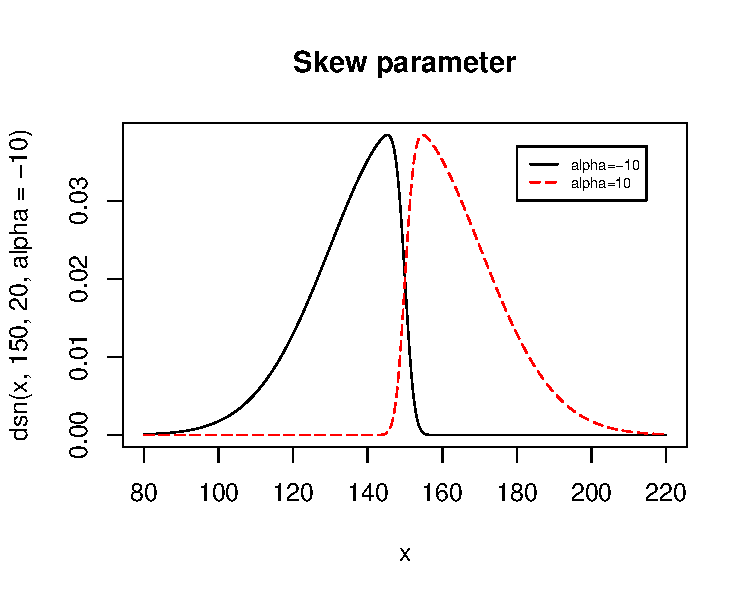
\includegraphics[width=.5\linewidth]{figure/dsn-1} 

\end{knitrout}
\end{center}

\noindent The parameter $S$ describes the total run size (the total number of fish passing the weir over the course of the run). Run sizes are really large, so they put the prior on $log(S)$. They used a normal prior, indicating that the log of the run size is somewhere between $7$ and $8$, which means that the total run size is somewhere between $1097$ and $2981$ fish. They call this a relatively flat prior for the total run size. I think a flat prior makes sense in this situation because run sizes do vary greatly from year to year. Since they intend to use this model for years and years, they truly do have little knowledge about what the run sizes will be in subsequent years (although they do have a general idea about the smallest and largest run sizes). \\

\noindent Lastly, there is the dispersion parameter for the negative binomial process variation model. They defined the first parameter in the negative binomial model as a function of $\theta$, $\lambda=\frac{\theta}{\theta+c_t}$. They chose this particular function for $\lambda$ because it allows the passage count variability to increase with the magnitude of the passage while keeping the mean at $c_t$, the daily passage count on day $t$. It took me a while to figure out what parameterization of the negative binomial distribution they were using. Thanks to Megan and the openBUGS helpfile, I figured out the mean of the given distribution is in fact $c_t$ and the variance is $c_t+\frac{c_t^2}{\theta}$. They chose a $Gam(0.1, 0.1)$ prior for $\theta$. I picked reasonable arbitrary values of $c_t$ and then explored the probable standard deviations, given the prior on $\theta$. See the plots below. The prior on $\theta$ suggests that values of $\theta$ between $0.5$ and $1.7$ are the most probable. If $c_t=20$, these values correspond to standard deviations between $16$ and $77$. If $c_t=100$, these values correspond to standard deviations between $77$ and $142$. I would say that this is a weakly informative prior; the range of probably standard deviations is pretty large. Although the range makes sense and seems reasonable, it doesn't seem like they are incorporating much prior knowledge.

\begin{center}
\begin{knitrout}\footnotesize
\definecolor{shadecolor}{rgb}{0.969, 0.969, 0.969}\color{fgcolor}
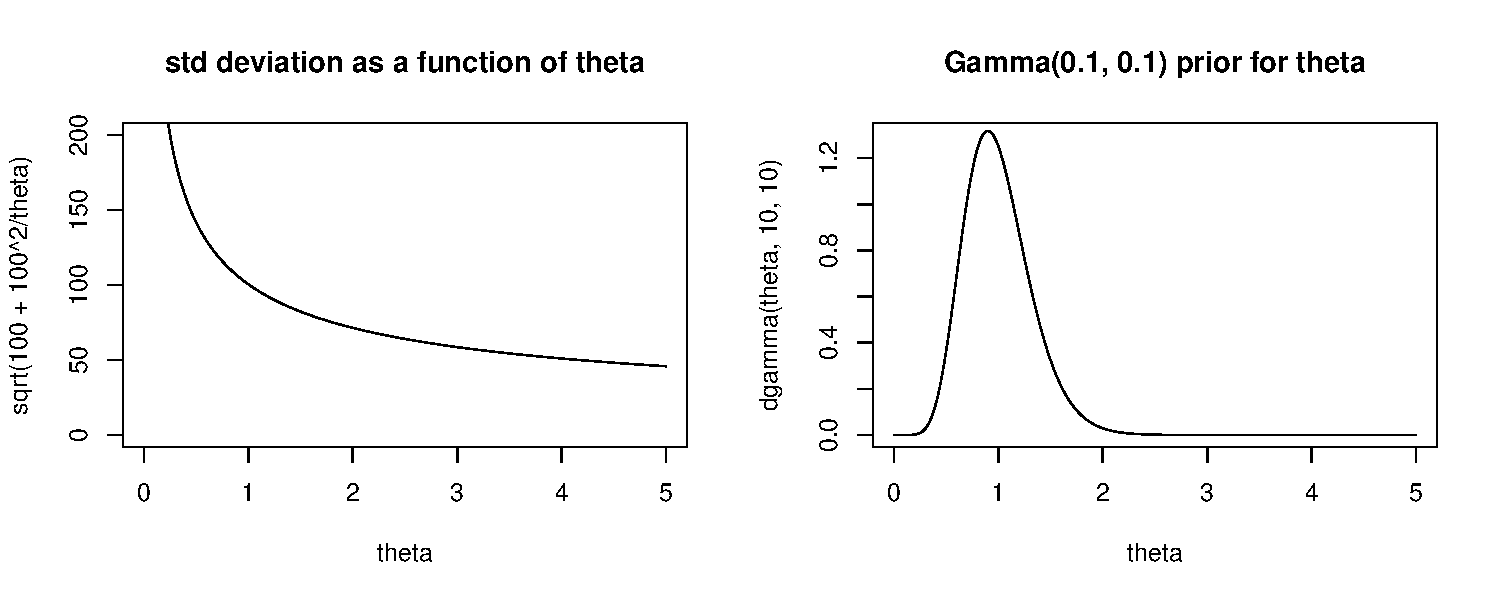
\includegraphics[width=\linewidth]{figure/lambda-1} 

\end{knitrout}
\end{center}

\newpage

\item There are difficulties both in deciding whether it is appropriate use a non-informative prior in a Bayesian analysis and then in choosing a prior that is always vague, but non-informative priors can be useful as long as you check that the posterior density is proper and not sensitive to the choice of prior.

\item \begin{enumerate}
\item Gelman's first argument for weakly informative priors is one of convenience; that it often is more convenient, mathematically, to use a weakly informative prior than a strongly informative one. For example, if we have a poisson likelihood, it's more convenient to choose a gamma prior, even if all of the information we have about the parameter can't be expressed as well with the gamma distribution as it could be with another distribution. He does mention here that ``arguments for convenience are best justified by the claim that the answer would not have changed much had we been more accurate.'' I do agree with this argument, but I think it's kind of strange that he doesn't emphasize the importance of doing a sensitivity analysis to check that the posterior is not sensitive to the choice of prior. He emphasizes this in the previous section on non-informative priors, but I would add that it is also important here, especially if he is using convenience as a main argument for using weakly informative priors. \\

In the next section, he mentions that maybe we don't always want to include all of the relevant information we have about a parameter in the prior. He mentions that you might not want the prior to pull the posterior in any pre-determined direction, especially if the goal of the study is to test a theory. This seems really weird to me, because if your goal is to test some theory, why wouldn't you go about the analysis from a frequentist perspective? It seems like a main strength of the Bayesian analysis is the ability to incorporate prior knowledge; but if you don't really want the prior knowledge to influence results, why would you be doing a Bayesian analysis at all? Even after discussing this in class, I'm not sure I completely agree with or understand the idea of moving the prior distribution in the opposite direction of your existing knowledge about the parameter in order to strengthen your results.

\item One option would be to start with a highly informative prior and then broaden it to incorporate more uncertainty. In this case, we could start with the prior they specified, a $Beta(2.3, 4.28)$ distribution. We could then add more probability in the tails to make it flatter and account for the prior knowledge that $12\%$ of the previous estimates were $1$. A second option would be to start with a $Unif(0, 1)$ prior and then change the shape slightly to account for there being more prior estimates between $0$ and $0.5$.

\end{enumerate}


\item I'm not sure this was the most computationally efficient way to do this, but I simply found the $50$th percentile and the $90$th percentile for beta distributions with many different combinations of $a$ and $b$. I then found the $a$ and $b$ that made the $50$th percentile closest to $0.3$ and the $90$th percentile closest to $0.75$. The beta distribution that I found was a $Beta(0.79, 1.47)$. The code and plot are shown below.
\begin{center}
\begin{singlespace}
\begin{knitrout}\footnotesize
\definecolor{shadecolor}{rgb}{0.969, 0.969, 0.969}\color{fgcolor}\begin{kframe}
\begin{alltt}
\hlcom{#define a, b and all combinations}
\hlstd{a} \hlkwb{<-} \hlkwd{seq}\hlstd{(}\hlnum{0.1}\hlstd{,}\hlnum{5}\hlstd{,}\hlnum{0.01}\hlstd{)}
\hlstd{b} \hlkwb{<-} \hlkwd{seq}\hlstd{(}\hlnum{0.1}\hlstd{,}\hlnum{5}\hlstd{,}\hlnum{0.01}\hlstd{)}
\hlstd{grid.vals} \hlkwb{<-} \hlkwd{expand.grid}\hlstd{(a, b)}

\hlcom{#function to evaluate the median}
\hlstd{median.fun} \hlkwb{<-} \hlkwa{function}\hlstd{(}\hlkwc{vec}\hlstd{) \{}\hlkwd{qbeta}\hlstd{(}\hlnum{0.5}\hlstd{, vec[}\hlnum{1}\hlstd{], vec[}\hlnum{2}\hlstd{])\}}

\hlcom{#find median at all combos of a and b and then subtract desired median of 0.3}
\hlstd{median} \hlkwb{<-} \hlkwd{matrix}\hlstd{(}\hlkwd{apply}\hlstd{(grid.vals,}\hlnum{1}\hlstd{, median.fun),} \hlkwc{nrow}\hlstd{=}\hlkwd{length}\hlstd{(a),} \hlkwc{ncol}\hlstd{=}\hlkwd{length}\hlstd{(b))}
\hlstd{median.min} \hlkwb{<-} \hlkwd{abs}\hlstd{(median}\hlopt{-}\hlnum{0.3}\hlstd{)}

\hlcom{#same process for 90th percentile}
\hlstd{fun.90} \hlkwb{<-} \hlkwa{function}\hlstd{(}\hlkwc{vec90}\hlstd{) \{}\hlkwd{qbeta}\hlstd{(}\hlnum{0.9}\hlstd{, vec90[}\hlnum{1}\hlstd{], vec90[}\hlnum{2}\hlstd{])\}}
\hlstd{perc.90} \hlkwb{<-} \hlkwd{matrix}\hlstd{(}\hlkwd{apply}\hlstd{(grid.vals,}\hlnum{1}\hlstd{, fun.90),} \hlkwc{nrow}\hlstd{=}\hlkwd{length}\hlstd{(a),} \hlkwc{ncol}\hlstd{=}\hlkwd{length}\hlstd{(b))}
\hlstd{min.90} \hlkwb{<-} \hlkwd{abs}\hlstd{(perc.90}\hlopt{-}\hlnum{0.75}\hlstd{)}

\hlcom{#find a and b that minimize the sum of the differences from 0.3 and 0.75}
\hlstd{sum} \hlkwb{<-} \hlstd{median.min}\hlopt{+}\hlstd{min.90}
\hlstd{a} \hlkwb{<-} \hlstd{a[}\hlkwd{which}\hlstd{(sum} \hlopt{==} \hlkwd{min}\hlstd{(sum),} \hlkwc{arr.ind} \hlstd{=} \hlnum{TRUE}\hlstd{)[}\hlnum{1}\hlstd{]]}
\hlstd{b} \hlkwb{<-} \hlstd{b[}\hlkwd{which}\hlstd{(sum} \hlopt{==} \hlkwd{min}\hlstd{(sum),} \hlkwc{arr.ind} \hlstd{=} \hlnum{TRUE}\hlstd{)[}\hlnum{2}\hlstd{]]}

\hlcom{#check that the a,b produce desired result}
\hlcom{#qbeta(.5, a, b) = 0.3000459}
\hlcom{#qbeta(.9, a, b) = 0.7507122}

\hlcom{#plot}
\hlstd{x} \hlkwb{<-} \hlkwd{seq}\hlstd{(}\hlnum{0}\hlstd{,} \hlnum{1}\hlstd{,} \hlkwc{by}\hlstd{=}\hlnum{0.01}\hlstd{)}
\hlkwd{plot}\hlstd{(x,} \hlkwd{dbeta}\hlstd{(x, a, b),} \hlkwc{type}\hlstd{=}\hlstr{"l"}\hlstd{,} \hlkwc{main}\hlstd{=}\hlstr{"Beta(0.79, 1.47)"}\hlstd{)}
\end{alltt}
\end{kframe}
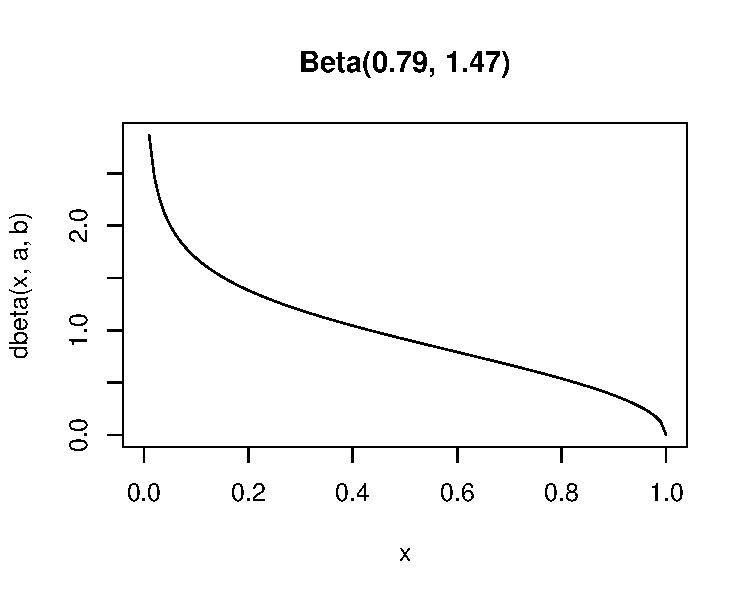
\includegraphics[width=0.5\linewidth]{figure/integrate-1} 

\end{knitrout}
\end{singlespace}
\end{center}

\item \begin{enumerate}

\item Suppose $x$ is fixed and $\lambda$ is unknown. Then,
\begin{align*}
p(\lambda|x) &= \frac{e^{-\lambda}\lambda^x}{x!} \\
&= \frac{e^{-1\lambda}1^{x+1}\lambda^{(x+1)-1}}{x!}
\end{align*}

This is a $Gam(x+1, 1)$ distribution where $x+1\geq0$ is fixed and $\lambda > 0$ is unknown. So, if we multiply a Poisson likelihood by a gamma prior, the posterior distribution will be a gamma as well.  In general, if $X \sim Poi(\lambda)$ and $\lambda \sim Gam(a, b)$, then posterior distribution of $\lambda|x$ is $Gam(x+a, b+1)$, for one draw from the $Poi(\lambda)$ distribution. See the proof below.
\begin{align*}
p(\lambda|x) &= \frac{p(x|\lambda)*p(\lambda)}{m(x)} \\
&= \frac{\frac{e^{-\lambda}\lambda^x}{x!}\frac{\lambda^{a-1}b^ae^{-b\lambda}}{\Gamma(a)}}{m(x)} \\
&= \frac{\frac{b^a}{x!\Gamma(a)}e^{-(b+1)\lambda}\lambda^{x+a-1}}{m(x)} \\
&\propto e^{-(b+1)\lambda}\lambda^{x+a-1} 
\end{align*}

Suppose $X$ follows a distribution that is a member of the exponential family, and suppose the prior for a parameter $\theta$ is also a member of the exponential family. Then, the posterior distribution is also a member of the exponential family. Just as we saw with the poisson and gamma distributions, if you multiply the pdf or pmf of an exponential family distribution by the pdf or pmf of another exponential family distribution, you will get back a member of the exponential family. See the proof below.
\begin{align*}
f(\theta|x) &\propto f(x|\theta)f(\theta) \\
&\propto h(x)c(\theta)e^{\sum_{i=1}^{n}w_i(\theta)t_i(x)}l(\theta)e^{\sum_{j=1}^{n_j}w_i(\theta)} \\
&\propto h(x)m(\theta)e^{\sum_{k=1}^{n_k}w_k(\theta)t_k(x)} 
\end{align*}

\item In part (a) I showed that for one draw from a $Poi(\lambda)$ distribution with a prior of $Gam(a,b)$, the posterior distribution is $Gam(x+a, b+1)$. Here, I show that for $n$ independent draws from a $Poi(\lambda)$, the posterior distribution is $Gam(\sum_{i=1}^nx_i+a, b+n)$. 
\begin{align*}
p(\lambda|x) &= \frac{p(x|\lambda)*p(\lambda)}{m(x)} \\
&= \frac{\frac{e^{-n\lambda}\lambda^{\sum x_i}}{\prod_{i=1}^nx_i!}\frac{\lambda^{a-1}b^ae^{-b\lambda}}{\Gamma(a)}}{\int_0^{\infty}\frac{e^{-n\lambda}\lambda^{\sum x_i}}{\prod_{i=1}^nx_i!}\frac{\lambda^{a-1}b^{a}e^{-b\lambda}}{\Gamma(a)}} \\
&= \frac{\frac{b^a}{\prod_{i=1}^nx_i!\Gamma(a)}e^{-(n+b)\lambda}\lambda^{\sum x_i+a-1}}{\frac{b^a\Gamma(\sum x_i+a)}{(1+b)^{\sum x_i+a}\prod_{i=1}^nx_i!\Gamma(a)}} \\
&= \frac{e^{-(n+b)\lambda}\lambda^{\sum x_i+a-1}(n+b)^{\sum x_i+a}}{\Gamma(\sum x_i+a)}
\end{align*}

\item From the likelihood, our estimate of the rate parameter is just $x$, the number of `successes' observed in one effort. For example, if we are a fishing trawler, and we put out our net once and get $5$ fish, we would estimate $\lambda$ to be $5$. The posterior mean for $\lambda$ given $x$ is $\frac{x+a}{b+1}$. If we observed $x=5$ and we start with a $Gam(1,1)$ prior, then the posterior mean for $\lambda$ is $6/2=3$. If we start with a $Gam(3,3)$ prior, then the posterior mean for $\lambda$ is $8/4=2$. We can think of this process as adding $a$ successful observations and increasing the total effort by $b$. For this example, we would be increasing the number of fish caught by $a$, but then we divide this over $b+1$ drops of the net.

\item I started by solving for possible values of $\alpha$ and $\beta$ that would make the mean of the distribution close to $20$ and the standard deviation close to $5$. I experimented with different values and found that a $Gam(20, 1)$ looked the best for the given conditions. Based on this distribution, the probability that $\lambda$ is less than $10$ or greater than $35$ is $0.00345+0.00232=0.00577$. The probability that $\lambda$ is between $10$ and $15$ or $25$ and $35$ is $0.1213+0.1313 = 0.2526$. The probability that $\lambda$ is between $15$ and $25$ is $0.7416$. I think this is a reasonable way to satisfy the constraints provided.

\begin{center}
\begin{knitrout}\footnotesize
\definecolor{shadecolor}{rgb}{0.969, 0.969, 0.969}\color{fgcolor}
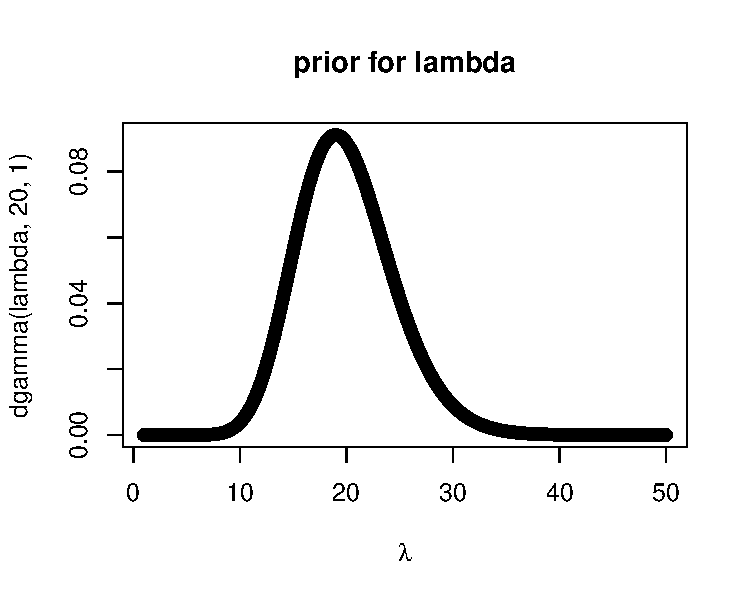
\includegraphics[width=0.5\linewidth]{figure/gammas-1} 

\end{knitrout}
\end{center}

\item I drew a $\lambda$ of $20.66$ and then drew $20$ independent observations from $Poi(20.66)$.

\begin{singlespace}
\begin{knitrout}\footnotesize
\definecolor{shadecolor}{rgb}{0.969, 0.969, 0.969}\color{fgcolor}\begin{kframe}
\begin{alltt}
\hlkwd{set.seed}\hlstd{(}\hlnum{15}\hlstd{)}
\hlstd{lambda.draw} \hlkwb{<-} \hlkwd{rgamma}\hlstd{(}\hlnum{1}\hlstd{,} \hlnum{20}\hlstd{,} \hlnum{1}\hlstd{)}
\hlstd{x.vec} \hlkwb{<-} \hlkwd{rpois}\hlstd{(}\hlnum{20}\hlstd{, lambda.draw)}
\end{alltt}
\end{kframe}
\end{knitrout}
\end{singlespace}

\item The plot of the observed data is below.

\begin{center}
\begin{knitrout}\footnotesize
\definecolor{shadecolor}{rgb}{0.969, 0.969, 0.969}\color{fgcolor}
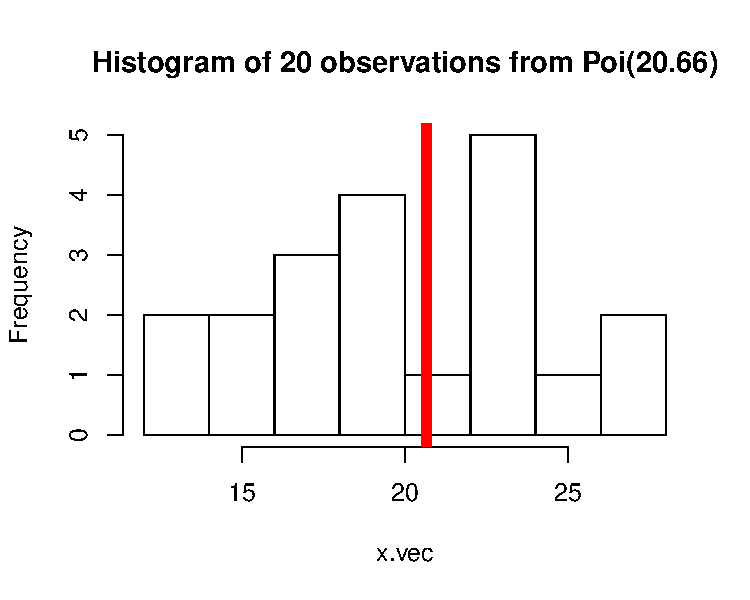
\includegraphics[width=0.5\linewidth]{figure/plotobs-1} 

\end{knitrout}
\end{center}

\item From (b), the posterior distribution of $\lambda|x$ is $Gam(\sum_{i=1}^nx_i+a, b+n)$ which is $Gam(409+20, 1+20)=Gam(429, 21)$. My work is below. I used numerical integration to sum under the likelihood curve, and then I used this number to normalize the likelihood.
\begin{align*}
p(\lambda|x) &= \frac{p(x|\lambda)*p(\lambda)}{m(x)} \\
&= \frac{\frac{e^{-20\lambda}\lambda^{409}}{\prod_{i=1}^{20}x_i!}\frac{\lambda^{19}1^19e^{-1\lambda}}{\Gamma(20)}}{\int_0^{\infty}\frac{e^{-20\lambda}\lambda^{409}}{\prod_{i=1}^{20}x_i!}\frac{\lambda^{19}1^{20}e^{-\lambda}}{\Gamma(20)}} \\
&= \frac{\frac{1}{\prod_{i=1}^{20}x_i!\Gamma(20)}e^{-(20+b)\lambda}\lambda^{409+19}}{\frac{\Gamma(409+20)}{(1+20)^{409+20}\prod_{i=1}^{20}x_i!\Gamma(20)}} \\
&= \frac{e^{-(21)\lambda}\lambda^{429-1}(21)^{429}}{\Gamma(429)}
\end{align*}

\begin{center}
\begin{knitrout}\footnotesize
\definecolor{shadecolor}{rgb}{0.969, 0.969, 0.969}\color{fgcolor}
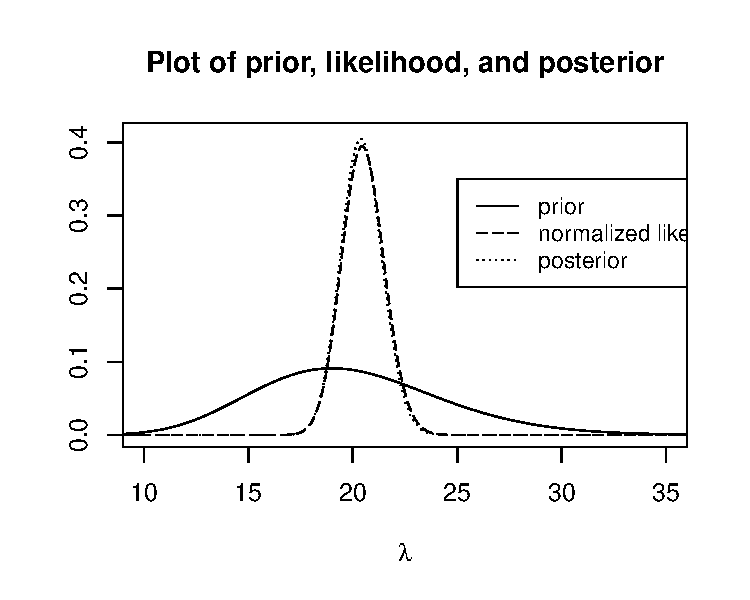
\includegraphics[width=0.7\linewidth]{figure/plotall-1} 

\end{knitrout}
\end{center}

\item The $90\%$ posterior interval for $\lambda$ is $(19.83, 22.41)$.
\begin{knitrout}\footnotesize
\definecolor{shadecolor}{rgb}{0.969, 0.969, 0.969}\color{fgcolor}\begin{kframe}
\begin{alltt}
\hlkwd{c}\hlstd{(}\hlkwd{qgamma}\hlstd{(}\hlnum{0.275}\hlstd{,} \hlnum{429}\hlstd{,} \hlnum{21}\hlstd{),} \hlkwd{qgamma}\hlstd{(}\hlnum{0.975}\hlstd{,} \hlnum{429}\hlstd{,} \hlnum{21}\hlstd{))}
\end{alltt}
\end{kframe}
\end{knitrout}

\item The posterior probability that $\lambda$ is between $10$ and $20$ is $0.337$.
\begin{knitrout}\footnotesize
\definecolor{shadecolor}{rgb}{0.969, 0.969, 0.969}\color{fgcolor}\begin{kframe}
\begin{alltt}
\hlkwd{pgamma}\hlstd{(}\hlnum{20}\hlstd{,} \hlnum{429}\hlstd{,} \hlnum{21}\hlstd{)}\hlopt{-}\hlkwd{pgamma}\hlstd{(}\hlnum{10}\hlstd{,} \hlnum{429}\hlstd{,} \hlnum{21}\hlstd{)}
\end{alltt}
\end{kframe}
\end{knitrout}

\item The posterior probability that $\lambda$ is less than $5$ is $7.65*10^{-124}$.
\begin{knitrout}\footnotesize
\definecolor{shadecolor}{rgb}{0.969, 0.969, 0.969}\color{fgcolor}\begin{kframe}
\begin{alltt}
\hlkwd{pgamma}\hlstd{(}\hlnum{5}\hlstd{,} \hlnum{429}\hlstd{,} \hlnum{21}\hlstd{)}
\end{alltt}
\end{kframe}
\end{knitrout}

\item The range of values drawn from the Poisson distribution was narrower when $\lambda$ was fixed, and the standard deviation was smaller. The range of the observations for the random $\lambda$ was $3$ to $44$, compared to a range of $9$ to $37$ for the fixed $\lambda$. The standard deviation of the observations for the random $\lambda$ was $6.39$ compared to $4.69$. These results reflect the fact that there are two sources of uncertainty reflected in the second histogram - both uncertainty in the value of $\lambda$, and uncertainty in the observation. The first histogram reflects only uncertainty in the value of the observations.\\

Also, The histograms happened to be centered around the same value, but this occured because the fixed value of $\lambda$ that was drawn was close to the mean of the prior distribution ($20$). 

\begin{knitrout}\footnotesize
\definecolor{shadecolor}{rgb}{0.969, 0.969, 0.969}\color{fgcolor}
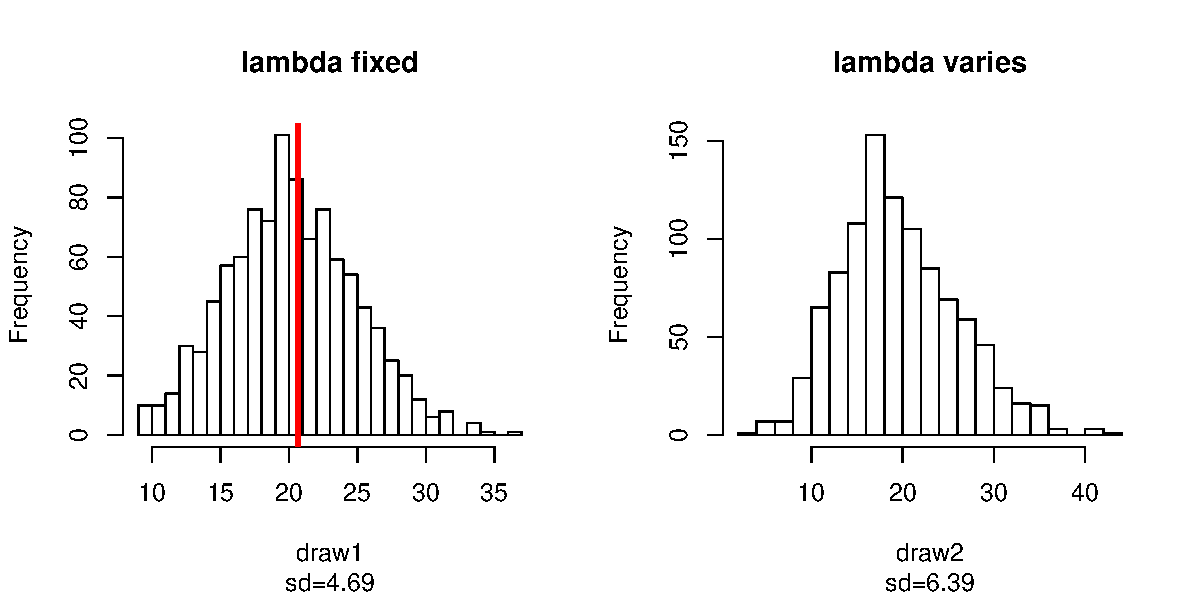
\includegraphics[width=\linewidth]{figure/draw-1} 

\end{knitrout}


\end{enumerate}

\item \begin{enumerate}
\item Gelman shows that for a binomial likelihood, the Jeffrey's prior on $\theta$ is $Beta(.5, .5)$. I do a transformation to find the kernel of the pdf of $\eta = logit(\theta)$.
\begin{align*}
\eta &= log(\frac{\theta}{1-\theta}) \hspace{.5in} \theta = \frac{e^{\eta}}{1+e^{\eta}} \\
f_{\eta}(\eta) &= f_{\theta}(\theta)*d\theta/d\eta \\
&= f_{\theta}(\frac{e^{\eta}}{1+e^{\eta}})*\frac{e^{\eta}}{(1+e^{\eta})^2} \\
&= \frac{(\frac{e^{\eta}}{1+e^{\eta}})^{-0.5}(\frac{1}{1+e^{\eta}})^{-0.5}\frac{e^{\eta}}{(1+e^{\eta})^2}}{\beta(0.5, 0.5)} \\
&\propto \frac{e^{\eta/2}}{1+e^{\eta}}
\end{align*}
where $\eta \in (-\infty, \infty)$. I then use R to find the normalizing constant to make the area under this curve sum to 1. In subsequent sections, I use the same code to find the normalizing constant.

\begin{center}
\begin{singlespace}
\begin{knitrout}\footnotesize
\definecolor{shadecolor}{rgb}{0.969, 0.969, 0.969}\color{fgcolor}\begin{kframe}
\begin{alltt}
\hlstd{etaprior} \hlkwb{<-} \hlkwa{function}\hlstd{(}\hlkwc{eta}\hlstd{) \{}
  \hlkwd{exp}\hlstd{(eta}\hlopt{/}\hlnum{2}\hlstd{)}\hlopt{/}\hlstd{(}\hlnum{1}\hlopt{+}\hlkwd{exp}\hlstd{(eta))}
\hlstd{\}}
\hlstd{eta} \hlkwb{<-} \hlkwd{seq}\hlstd{(}\hlopt{-}\hlnum{10}\hlstd{,} \hlnum{10}\hlstd{,} \hlkwc{by}\hlstd{=}\hlnum{0.0001}\hlstd{)}
\hlstd{y} \hlkwb{<-} \hlnum{0.0001}\hlopt{*}\hlkwd{etaprior}\hlstd{(eta)}
\hlstd{numint} \hlkwb{<-} \hlkwd{sum}\hlstd{(y)}
\hlkwd{plot}\hlstd{(eta,} \hlkwd{etaprior}\hlstd{(eta)}\hlopt{/}\hlstd{numint,} \hlkwc{type}\hlstd{=}\hlstr{"l"}\hlstd{,} \hlkwc{main}\hlstd{=}\hlstr{"normalized prior for eta=logit(theta)"}\hlstd{,} \hlkwc{xlab}\hlstd{=}\hlkwd{expression}\hlstd{(eta))}
\end{alltt}
\end{kframe}
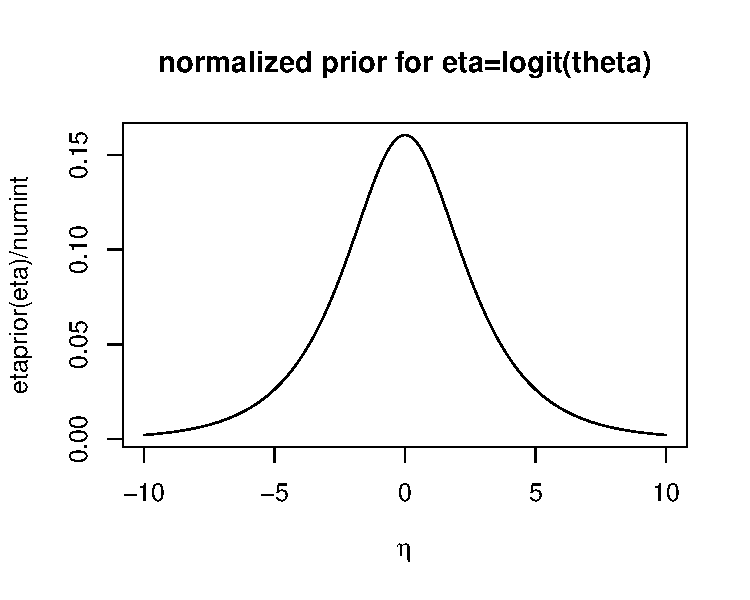
\includegraphics[width=.5\linewidth]{figure/plotprior1-1} 

\end{knitrout}
\end{singlespace}
\end{center}

\item The R function to calculate the likelihood and the plot of the likelihood is shown below.
\begin{singlespace}
\begin{knitrout}\footnotesize
\definecolor{shadecolor}{rgb}{0.969, 0.969, 0.969}\color{fgcolor}\begin{kframe}
\begin{alltt}
\hlstd{etalike} \hlkwb{<-} \hlkwa{function}\hlstd{(}\hlkwc{eta}\hlstd{)\{}
  \hlkwd{choose}\hlstd{(}\hlnum{30}\hlstd{,} \hlnum{8}\hlstd{)}\hlopt{*}\hlstd{(}\hlkwd{exp}\hlstd{(eta)}\hlopt{/}\hlstd{(}\hlnum{1}\hlopt{+}\hlkwd{exp}\hlstd{(eta)))}\hlopt{^}\hlnum{8}\hlopt{*}\hlstd{(}\hlnum{1}\hlopt{/}\hlstd{(}\hlnum{1}\hlopt{+}\hlkwd{exp}\hlstd{(eta)))}\hlopt{^}\hlnum{22}
\hlstd{\}}
\end{alltt}
\end{kframe}
\end{knitrout}
\end{singlespace}

\begin{center}
\begin{knitrout}\footnotesize
\definecolor{shadecolor}{rgb}{0.969, 0.969, 0.969}\color{fgcolor}
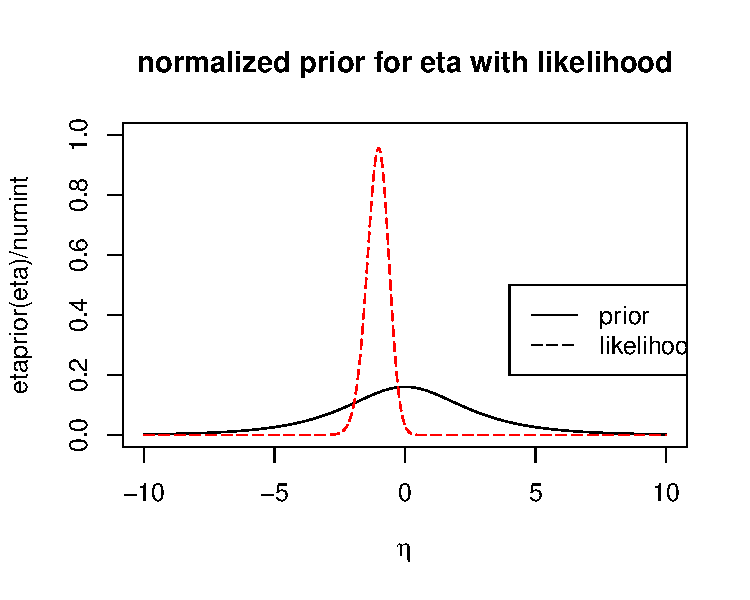
\includegraphics[width=.5\linewidth]{figure/likeeta-1} 

\end{knitrout}
\end{center}

\item The plot of the normalized prior, likelihood, and posterior is shown below. I am not surprised that the posterior distribution looks almost exactly like the likelihood. The prior is pretty flat, allowing the data to dominate, and the prior is centered near the likelihood. 
\begin{align*}
f(\eta|x=8) &\propto {30 \choose 8}(\frac{e^{\eta}}{1+e^{\eta}})^8(\frac{1}{1+e^{\eta}})^{22} \frac{e^{\eta/2}}{1+e^{\eta}} \\
&\propto \frac{e^{17\eta/2}}{(1+e^{\eta})^{31}}
\end{align*}



\begin{center}
\begin{knitrout}\footnotesize
\definecolor{shadecolor}{rgb}{0.969, 0.969, 0.969}\color{fgcolor}
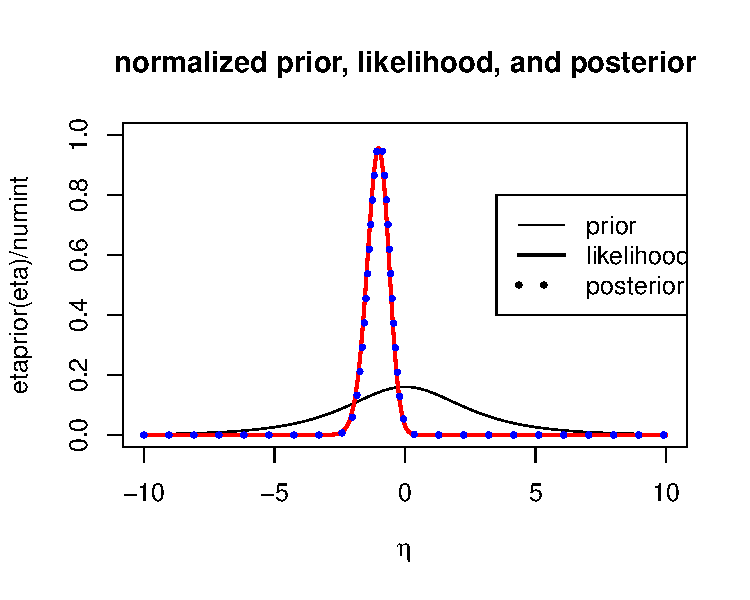
\includegraphics[width=.5\linewidth]{figure/posterior-1} 

\end{knitrout}
\end{center}

\item Using previous results, the posterior distribution for $\theta$ is a $Beta(8.5, 22.5)$. The posterior distribution found in (c) approximates the histogram created here. This shows that it is equivalent to find the posterior for $\eta$ itself or find the posterior for $\theta$ and then solve for $\eta$.

\begin{center}
\begin{knitrout}\footnotesize
\definecolor{shadecolor}{rgb}{0.969, 0.969, 0.969}\color{fgcolor}
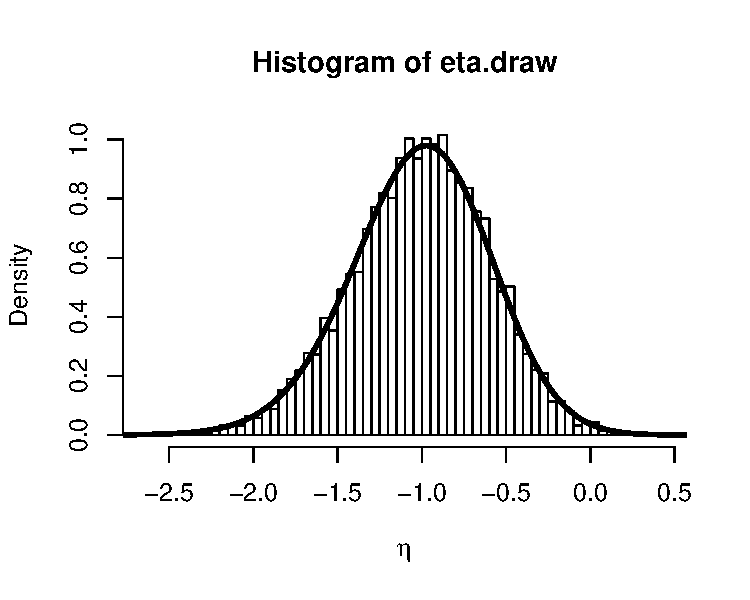
\includegraphics[width=.5\linewidth]{figure/backtotheta-1} 

\end{knitrout}
\end{center}

\item \begin{enumerate}
\item The prior distribution on $\theta$ is $Unif(0, 1)$, and the prior distribution on $\eta$ is an improper uniform distribution over the whole real line so that $f(\eta)=I(\eta)_{(-\infty, \infty)}$. 
\begin{knitrout}\footnotesize
\definecolor{shadecolor}{rgb}{0.969, 0.969, 0.969}\color{fgcolor}
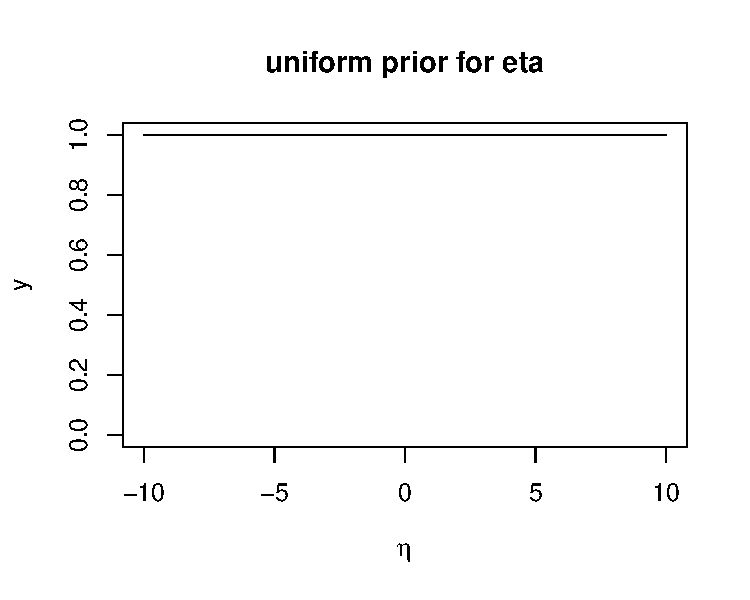
\includegraphics[width=.5\linewidth]{figure/etauniformprior-1} 

\end{knitrout}

\item The likelihood function is the same as part (b) and is plotted with the prior below.
\begin{knitrout}\footnotesize
\definecolor{shadecolor}{rgb}{0.969, 0.969, 0.969}\color{fgcolor}
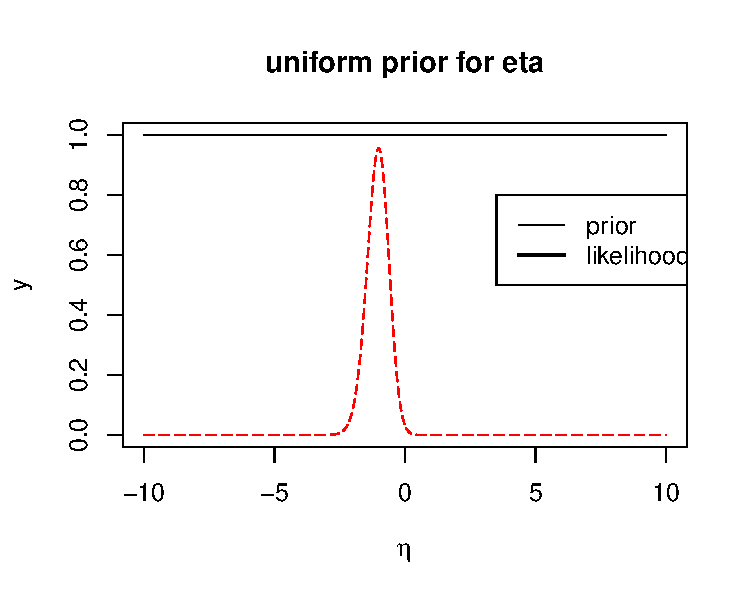
\includegraphics[width=.5\linewidth]{figure/etauniformlike-1} 

\end{knitrout}

\item Because the prior distribution for $\eta$ is uniform over the whole real line, the posterior distribution for $\eta$ is just the normalized likelihood. See work below.
\begin{align*}
\eta|x &\propto {30 \choose 8}(\frac{e^{\eta}}{1+e^{\eta}})^8(\frac{1}{1+e^{\eta}})^{22}I(\eta)_{(-\infty,\infty)} 
\end{align*}


\begin{knitrout}\footnotesize
\definecolor{shadecolor}{rgb}{0.969, 0.969, 0.969}\color{fgcolor}
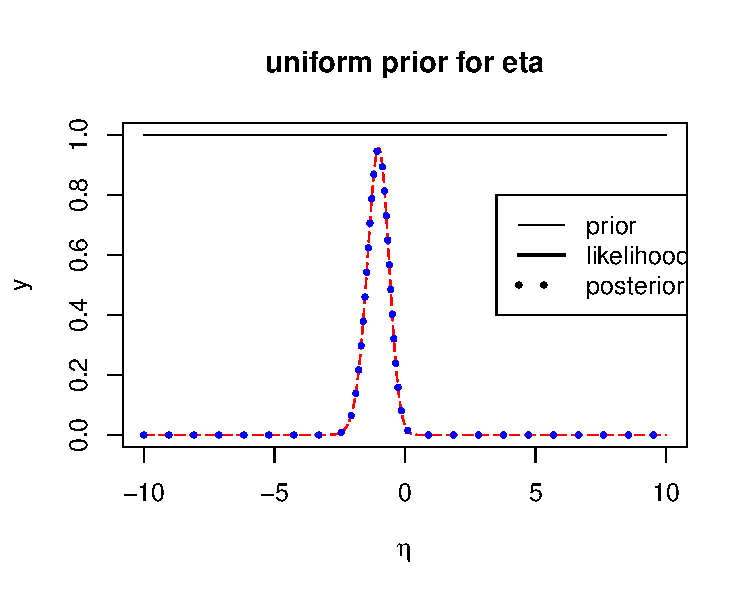
\includegraphics[width=.5\linewidth]{figure/etauniform-1} 

\end{knitrout}

\item I show below that the posterior distribution for $\theta$ is $Beta(9, 23)$. 
\begin{align*}
\theta|x &\propto \theta^8(1-\theta)^{22}I(\theta)_{(0,1)} \\
&\propto \theta^{9-1}(1-\theta)^{23-1}I(\theta)_{(0,1)} 
\end{align*}

I obtain $10000$ independent draws from a $Beta(9,23)$, and then I calculate $\eta$ for each draw. It turns out that the histogram of draws does not match up exactly with the posterior distribution for $\eta$ found by starting with a uniform prior on $\eta$. I think this shows that you can't just slap a flat prior on $\theta$ and a flat prior $\eta$ and expect to get the same results. A flat uniform prior will give us different results depending on what parameterization of $\theta$ we apply the prior to. If we really want to express the same beliefs by applying a prior to $\theta$ or a prior to a transformed version of $\theta$, we need to start with a Jeffrey's prior for $\theta$ then do the transformation to find the prior for the transformed version of $\theta$. 


\begin{center}
\begin{knitrout}\footnotesize
\definecolor{shadecolor}{rgb}{0.969, 0.969, 0.969}\color{fgcolor}
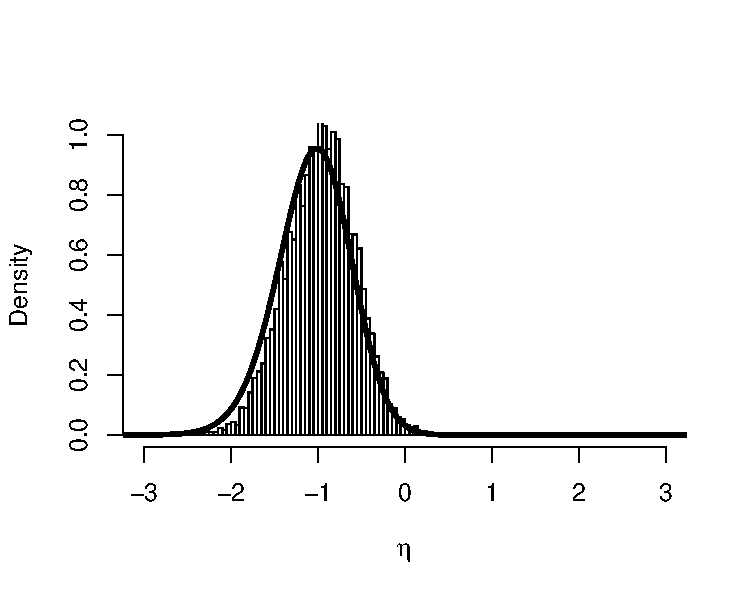
\includegraphics[width=.5\linewidth]{figure/backtouniftheta-1} 

\end{knitrout}
\end{center}

\end{enumerate}

\item If we start with a $Beta(0, 0)$ prior on $\theta$, the posterior distribution for $\theta$ is $Beta(8, 22)$. I obtained $10000$ draws from a $Beta(8, 22)$, and it matched up pretty closely with the posterior of $\eta$ obtained from the uniform prior on $\eta$. 

\begin{center}
\begin{knitrout}\footnotesize
\definecolor{shadecolor}{rgb}{0.969, 0.969, 0.969}\color{fgcolor}
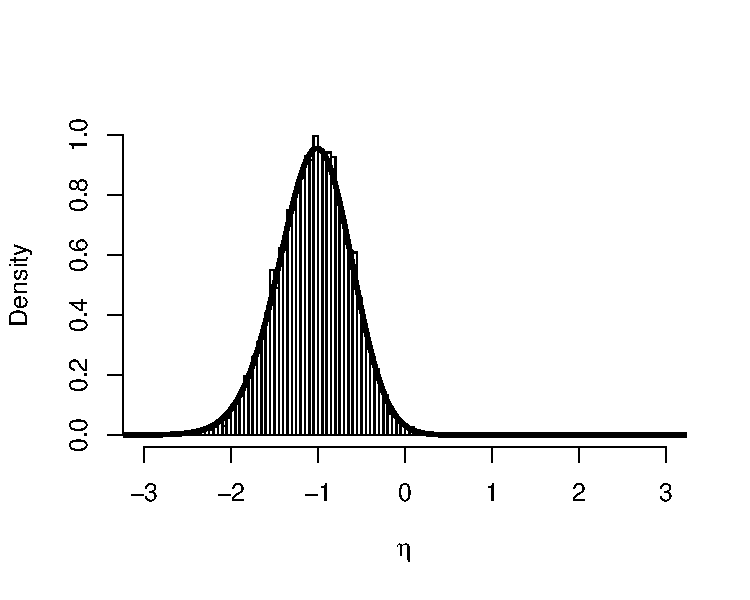
\includegraphics[width=.5\linewidth]{figure/backtounifthetabet00-1} 

\end{knitrout}
\end{center}

Seeing this, I went back and wondered what would happen if we started with a $Beta(0,0)$ prior on $\theta$ and then transformed to find the prior for $\eta$. It turns out that, after transformation, the prior for $\eta$ is the improper uniform distribution over the whole real line! See my work below. Even though the $Beta(0, 0)$ distribution is improper, it does follow Jeffrey's principle. We get the same result whether we use the $Beta(0, 0)$ prior for $\theta$ or whether we use the improper uniform prior on $\eta$.

\begin{align*}
\eta &= log(\frac{\theta}{1-\theta}) \hspace{.5in} \theta = \frac{e^{\eta}}{1+e^{\eta}} \\
f_{\eta}(\eta) &= f_{\theta}(\theta)*d\theta/d\eta \\
&= f_{\theta}(\frac{e^{\eta}}{1+e^{\eta}})*\frac{e^{\eta}}{(1+e^{\eta})^2} \\
&= \frac{(\frac{e^{\eta}}{1+e^{\eta}})^{-1}(\frac{1}{1+e^{\eta}})^{-1}\frac{e^{\eta}}{(1+e^{\eta})^2}}{\beta(0.5, 0.5)} \\
&\propto 1I(\eta)_{(-\infty, \infty)}
\end{align*}

\item I constructed a $92\%$ Wald confidence interval for $\theta$ by hand, $0.267 \pm 1.75\sqrt{0.267*0.733/30} = (0.126, 0.408)$. The posterior intervals under the given priors are shown in the following table.
\begin{table}[!h]
\centering
\begin{tabular}{c|c|c|c}
Prior & $92\%$ posterior & posterior interval & width of interval \\
\hline
Wald interval & & (0.126, 0.408) & 0.282 \\
Beta(0, 0) & Beta(8, 22) & (0.139, 0.416) & 0.277 \\
Beta(0.5, 0.5) & Beta(8.5, 22.5) & (0.147, 0.422) & 0.275\\
Beta(1, 1) & Beta(9, 23) & (0.154, 0.427) & 0.273\\
\hline
\end{tabular}
\end{table}

The $Beta(0, 0)$ prior gives an interval that is closest to the Wald interval. I am actually surprised that the interval from the $Beta(0,0)$ prior isn't closer to the Wald interval, because I think that if you use a non-informative prior, inference should be similar to what a frequentist would find. The Wald interval isn't completely trustworthy because the normal approximation may not be very good with a relatively small sample size of $30$, so I experimented to see if the Wald interval is closer to the $Beta(0,0)$ interval for larger sample sizes. If we increase the sample size to $80$, the Wald interval for $\theta$ is actually $(0.222, 0.311)$, which is very close to the $Beta(0, 0)$ interval of $(0.223, 0.312)$. \\

Also, the Wald interval is wider than the posterior intervals, and among the posterior intervals, the widths decrease as the posterior parameters increase. Also, the intervals are shifted farther right as the posterior parameters increase, reflecting the contribution of the prior. For a symmetric $Beta$ distribution, it will always be true that the posterior distribution gets pulled towards $0.5$ because the $Beta(\alpha, \alpha)$ prior adds $\alpha$ successes and $\alpha$ failures to what was observed.

\end{enumerate}

\item Next page.
\newpage
...
\newpage

\item \begin{enumerate}
\item Yes. I show below that the resulting posterior distribution is a $Beta(10, 40)$ which is a proper distribution.
\begin{align*}
\theta|x &\propto \theta^{10}(1-\theta)^{30}\theta^{-1}(1-\theta)^{-1}I(\theta)_{(0,1)} \\
&\propto \theta^{10-1}(1-\theta)^{30-1}I(\theta)_{(0,1)} 
\end{align*}

\item No. I show below that if we observe $0$ or $40$ successes, the resulting Beta distribution would have a parameter that is $0$. Since both parameters in the Beta distribution must be greater than $0$, this is not a proper distribution. 
\begin{align*}
\theta|x &\propto \theta^{0}(1-\theta)^{40}\theta^{-1}(1-\theta)^{-1}I(\theta)_{(0,1)} \\
&\propto \theta^{0-1}(1-\theta)^{40-1}I(\theta)_{(0,1)} \\
\theta|x &\propto \theta^{40}(1-\theta)^{0}\theta^{-1}(1-\theta)^{-1}I(\theta)_{(0,1)} \\
&\propto \theta^{40-1}(1-\theta)^{0-1}I(\theta)_{(0,1)} 
\end{align*}

In the code below, I find the area under the $Beta(10, 40)$ distribution by numerical integration. It sums to $1$ and is a proper distribution.
\begin{singlespace}
\begin{knitrout}\footnotesize
\definecolor{shadecolor}{rgb}{0.969, 0.969, 0.969}\color{fgcolor}\begin{kframe}
\begin{alltt}
\hlcom{#define the support of the beta distribtuion}
\hlstd{x} \hlkwb{<-} \hlkwd{seq}\hlstd{(}\hlnum{0}\hlstd{,} \hlnum{0.9999}\hlstd{,} \hlkwc{by}\hlstd{=}\hlnum{0.0001}\hlstd{)}
\hlcom{#left hand riemann sum}
\hlstd{is.pdf} \hlkwb{<-} \hlnum{0.0001}\hlopt{*}\hlkwd{dbeta}\hlstd{(x,} \hlnum{10}\hlstd{,} \hlnum{40}\hlstd{)}
\hlcom{#sum(is.pdf)=1}
\end{alltt}
\end{kframe}
\end{knitrout}
\end{singlespace}

In the code below, I find the area under the $Beta(0, 40)$ and $Beta(40, 0)$ curves by numerical integration. We can see that both curves are just horizontal lines at $0$. I find the area under the $0$ successes curve to be infinite, and I find the area under the $40$ successes curve to be $0$.

\begin{singlespace}
\begin{knitrout}\footnotesize
\definecolor{shadecolor}{rgb}{0.969, 0.969, 0.969}\color{fgcolor}\begin{kframe}
\begin{alltt}
\hlcom{#define the support of the beta distribtuion}
\hlstd{x} \hlkwb{<-} \hlkwd{seq}\hlstd{(}\hlnum{0}\hlstd{,} \hlnum{0.9999}\hlstd{,} \hlkwc{by}\hlstd{=}\hlnum{0.0001}\hlstd{)}
\hlcom{#left hand riemann sum}
\hlstd{is.pdf0} \hlkwb{<-} \hlnum{0.0001}\hlopt{*}\hlkwd{dbeta}\hlstd{(x,} \hlnum{0}\hlstd{,} \hlnum{40}\hlstd{)}
\hlcom{#sum(is.pdf0)=Inf}
\hlkwd{plot}\hlstd{(x,} \hlkwd{dbeta}\hlstd{(x,} \hlnum{0}\hlstd{,} \hlnum{40}\hlstd{),} \hlkwc{type}\hlstd{=}\hlstr{"l"}\hlstd{,} \hlkwc{main}\hlstd{=}\hlstr{"0 successes"}\hlstd{)}
\end{alltt}
\end{kframe}
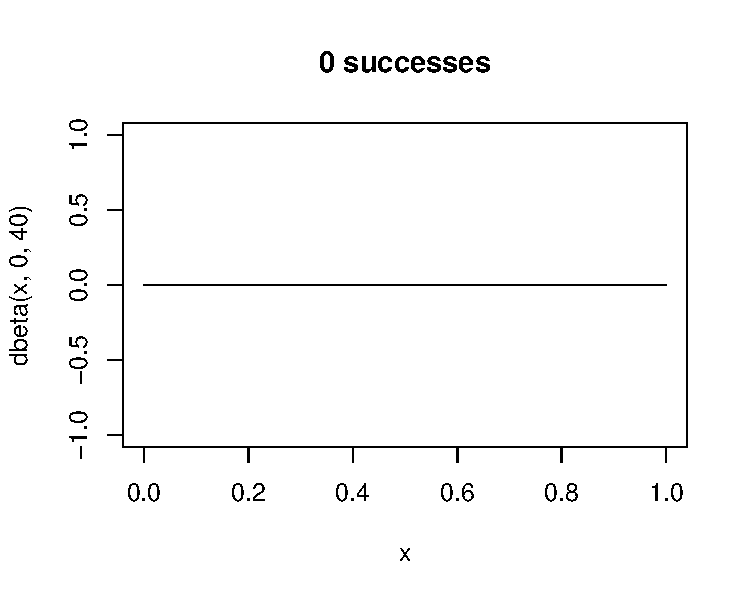
\includegraphics[width=.5\linewidth]{figure/numint3-1} 
\begin{kframe}\begin{alltt}
\hlcom{#define the support of the beta distribtuion}
\hlstd{x} \hlkwb{<-} \hlkwd{seq}\hlstd{(}\hlnum{0}\hlstd{,} \hlnum{0.9999}\hlstd{,} \hlkwc{by}\hlstd{=}\hlnum{0.0001}\hlstd{)}
\hlcom{#left hand riemann sum}
\hlstd{is.pdf40} \hlkwb{<-} \hlnum{0.0001}\hlopt{*}\hlkwd{dbeta}\hlstd{(x,} \hlnum{40}\hlstd{,} \hlnum{0}\hlstd{)}
\hlcom{#sum(is.pdf40)=0}
\hlkwd{plot}\hlstd{(x,} \hlkwd{dbeta}\hlstd{(x,} \hlnum{40}\hlstd{,} \hlnum{0}\hlstd{),} \hlkwc{type}\hlstd{=}\hlstr{"l"}\hlstd{,} \hlkwc{main}\hlstd{=}\hlstr{"40 successes"}\hlstd{)}
\end{alltt}
\end{kframe}
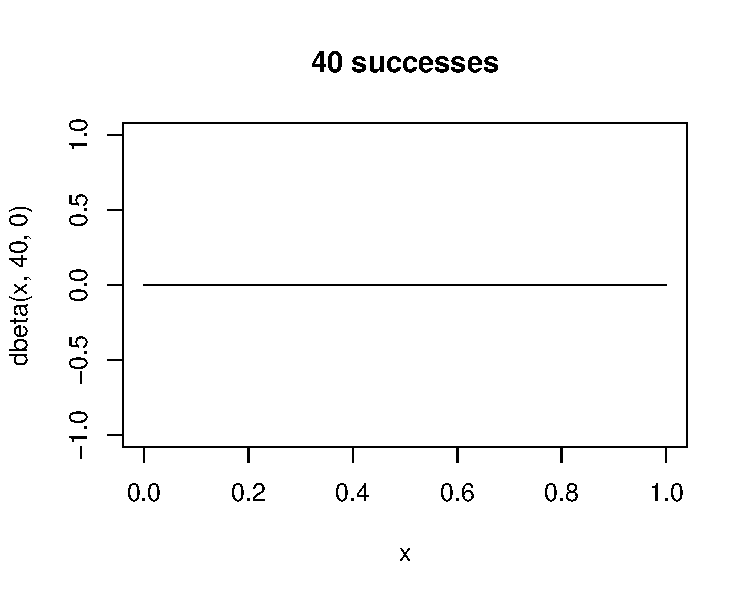
\includegraphics[width=.5\linewidth]{figure/numint3-2} 

\end{knitrout}
\end{singlespace}

I think this is really interesting because in part (a) we started with an improper prior and ended up with a proper posterior. In part (b), however, we started with an improper prior and ended up with an improper posterior. I think the lesson here is that sometimes you can use an improper prior distribution, and sometimes you can't. You just have to put in the work to check that the resulting posterior distribution is proper.


\end{enumerate}

\end{enumerate}
\end{doublespacing}

\newpage
{\bf \large R code appendix}

\begin{knitrout}\footnotesize
\definecolor{shadecolor}{rgb}{0.969, 0.969, 0.969}\color{fgcolor}\begin{kframe}
\begin{alltt}
\hlkwd{require}\hlstd{(sn)}
\hlstd{x} \hlkwb{<-} \hlkwd{seq}\hlstd{(}\hlnum{80}\hlstd{,} \hlnum{220}\hlstd{,} \hlkwc{by}\hlstd{=}\hlnum{0.01}\hlstd{)}
\hlkwd{plot}\hlstd{(x,} \hlkwd{dsn}\hlstd{(x,} \hlnum{150}\hlstd{,} \hlnum{20}\hlstd{,} \hlkwc{alpha}\hlstd{=}\hlopt{-}\hlnum{10}\hlstd{),} \hlkwc{type}\hlstd{=}\hlstr{"l"}\hlstd{,} \hlkwc{main}\hlstd{=}\hlstr{"Skew parameter"}\hlstd{)}
\hlkwd{lines}\hlstd{(x,} \hlkwd{dsn}\hlstd{(x,} \hlnum{150}\hlstd{,} \hlnum{20}\hlstd{,} \hlkwc{alpha}\hlstd{=}\hlnum{10}\hlstd{),} \hlkwc{col}\hlstd{=}\hlstr{"red"}\hlstd{,} \hlkwc{lty}\hlstd{=}\hlnum{5}\hlstd{)}
\hlkwd{legend}\hlstd{(}\hlnum{180}\hlstd{,} \hlnum{0.037}\hlstd{,} \hlkwd{c}\hlstd{(}\hlstr{"alpha=-10"}\hlstd{,} \hlstr{"alpha=10"}\hlstd{),} \hlkwc{lty}\hlstd{=}\hlkwd{c}\hlstd{(}\hlnum{1}\hlstd{,}\hlnum{5}\hlstd{),} \hlkwc{col}\hlstd{=}\hlkwd{c}\hlstd{(}\hlstr{"black"}\hlstd{,} \hlstr{"red"}\hlstd{),} \hlkwc{cex}\hlstd{=}\hlnum{0.6}\hlstd{)}
\end{alltt}
\end{kframe}
\end{knitrout}

\begin{knitrout}\footnotesize
\definecolor{shadecolor}{rgb}{0.969, 0.969, 0.969}\color{fgcolor}\begin{kframe}
\begin{alltt}
\hlkwd{par}\hlstd{(}\hlkwc{mfrow}\hlstd{=}\hlkwd{c}\hlstd{(}\hlnum{1}\hlstd{,}\hlnum{2}\hlstd{))}
\hlstd{theta} \hlkwb{<-} \hlkwd{seq}\hlstd{(}\hlnum{0}\hlstd{,} \hlnum{5}\hlstd{,} \hlkwc{by}\hlstd{=}\hlnum{0.01}\hlstd{)}
\hlkwd{plot}\hlstd{(theta,} \hlkwd{sqrt}\hlstd{(}\hlnum{100}\hlopt{+}\hlnum{100}\hlopt{^}\hlnum{2}\hlopt{/}\hlstd{theta),} \hlkwc{main}\hlstd{=}\hlstr{"std deviation as a function of theta"}\hlstd{,} \hlkwc{type}\hlstd{=}\hlstr{"l"}\hlstd{,} \hlkwc{ylim}\hlstd{=}\hlkwd{c}\hlstd{(}\hlnum{0}\hlstd{,} \hlnum{200}\hlstd{))}
\hlkwd{plot}\hlstd{(theta,} \hlkwd{dgamma}\hlstd{(theta,} \hlnum{10}\hlstd{,} \hlnum{10}\hlstd{),} \hlkwc{type}\hlstd{=}\hlstr{"l"}\hlstd{,} \hlkwc{ylim}\hlstd{=}\hlkwd{c}\hlstd{(}\hlnum{0}\hlstd{,} \hlnum{1.3}\hlstd{),} \hlkwc{main}\hlstd{=}\hlstr{"Gamma(0.1, 0.1) prior for theta"}\hlstd{)}
\end{alltt}
\end{kframe}
\end{knitrout}

\begin{knitrout}\footnotesize
\definecolor{shadecolor}{rgb}{0.969, 0.969, 0.969}\color{fgcolor}\begin{kframe}
\begin{alltt}
\hlcom{#define a, b and all combinations}
\hlstd{a} \hlkwb{<-} \hlkwd{seq}\hlstd{(}\hlnum{0.1}\hlstd{,}\hlnum{5}\hlstd{,}\hlnum{0.01}\hlstd{)}
\hlstd{b} \hlkwb{<-} \hlkwd{seq}\hlstd{(}\hlnum{0.1}\hlstd{,}\hlnum{5}\hlstd{,}\hlnum{0.01}\hlstd{)}
\hlstd{grid.vals} \hlkwb{<-} \hlkwd{expand.grid}\hlstd{(a, b)}

\hlcom{#function to evaluate the median}
\hlstd{median.fun} \hlkwb{<-} \hlkwa{function}\hlstd{(}\hlkwc{vec}\hlstd{) \{}\hlkwd{qbeta}\hlstd{(}\hlnum{0.5}\hlstd{, vec[}\hlnum{1}\hlstd{], vec[}\hlnum{2}\hlstd{])\}}

\hlcom{#find median at all combos of a and b and then subtract desired median of 0.3}
\hlstd{median} \hlkwb{<-} \hlkwd{matrix}\hlstd{(}\hlkwd{apply}\hlstd{(grid.vals,}\hlnum{1}\hlstd{, median.fun),} \hlkwc{nrow}\hlstd{=}\hlkwd{length}\hlstd{(a),} \hlkwc{ncol}\hlstd{=}\hlkwd{length}\hlstd{(b))}
\hlstd{median.min} \hlkwb{<-} \hlkwd{abs}\hlstd{(median}\hlopt{-}\hlnum{0.3}\hlstd{)}

\hlcom{#same process for 90th percentile}
\hlstd{fun.90} \hlkwb{<-} \hlkwa{function}\hlstd{(}\hlkwc{vec90}\hlstd{) \{}\hlkwd{qbeta}\hlstd{(}\hlnum{0.9}\hlstd{, vec90[}\hlnum{1}\hlstd{], vec90[}\hlnum{2}\hlstd{])\}}
\hlstd{perc.90} \hlkwb{<-} \hlkwd{matrix}\hlstd{(}\hlkwd{apply}\hlstd{(grid.vals,}\hlnum{1}\hlstd{, fun.90),} \hlkwc{nrow}\hlstd{=}\hlkwd{length}\hlstd{(a),} \hlkwc{ncol}\hlstd{=}\hlkwd{length}\hlstd{(b))}
\hlstd{min.90} \hlkwb{<-} \hlkwd{abs}\hlstd{(perc.90}\hlopt{-}\hlnum{0.75}\hlstd{)}

\hlcom{#find a and b that minimize the sum of the differences from 0.3 and 0.75}
\hlstd{sum} \hlkwb{<-} \hlstd{median.min}\hlopt{+}\hlstd{min.90}
\hlstd{a} \hlkwb{<-} \hlstd{a[}\hlkwd{which}\hlstd{(sum} \hlopt{==} \hlkwd{min}\hlstd{(sum),} \hlkwc{arr.ind} \hlstd{=} \hlnum{TRUE}\hlstd{)[}\hlnum{1}\hlstd{]]}
\hlstd{b} \hlkwb{<-} \hlstd{b[}\hlkwd{which}\hlstd{(sum} \hlopt{==} \hlkwd{min}\hlstd{(sum),} \hlkwc{arr.ind} \hlstd{=} \hlnum{TRUE}\hlstd{)[}\hlnum{2}\hlstd{]]}

\hlcom{#check that the a,b produce desired result}
\hlcom{#qbeta(.5, a, b) = 0.3000459}
\hlcom{#qbeta(.9, a, b) = 0.7507122}

\hlcom{#plot}
\hlstd{x} \hlkwb{<-} \hlkwd{seq}\hlstd{(}\hlnum{0}\hlstd{,} \hlnum{1}\hlstd{,} \hlkwc{by}\hlstd{=}\hlnum{0.01}\hlstd{)}
\hlkwd{plot}\hlstd{(x,} \hlkwd{dbeta}\hlstd{(x, a, b),} \hlkwc{type}\hlstd{=}\hlstr{"l"}\hlstd{,} \hlkwc{main}\hlstd{=}\hlstr{"Beta(0.79, 1.47)"}\hlstd{)}
\end{alltt}
\end{kframe}
\end{knitrout}

\begin{knitrout}\footnotesize
\definecolor{shadecolor}{rgb}{0.969, 0.969, 0.969}\color{fgcolor}\begin{kframe}
\begin{alltt}
\hlstd{lambda} \hlkwb{<-} \hlkwd{seq}\hlstd{(}\hlnum{1}\hlstd{,}\hlnum{50}\hlstd{,} \hlkwc{by}\hlstd{=}\hlnum{0.01}\hlstd{)}
\hlcom{#plot(x, dgamma(x, 40,2))}
\hlcom{#plot(x, dgamma(x, 400/15,20/15))}
\hlkwd{plot}\hlstd{(lambda,} \hlkwd{dgamma}\hlstd{(lambda,} \hlnum{20}\hlstd{,} \hlnum{1}\hlstd{),} \hlkwc{xlab}\hlstd{=}\hlkwd{expression}\hlstd{(lambda),} \hlkwc{main}\hlstd{=}\hlstr{"prior for lambda"}\hlstd{)}
\hlcom{#pgamma(10, 20, 1)}
\hlcom{#1-pgamma(35,20,1)}
\hlcom{#pgamma(15, 20, 1) - pgamma(10, 20, 1)}
\hlcom{#pgamma(35, 20, 1) - pgamma(25, 20, 1)}
\hlcom{#pgamma(25, 20, 1) - pgamma(15, 20, 1)}
\end{alltt}
\end{kframe}
\end{knitrout}

\begin{knitrout}\footnotesize
\definecolor{shadecolor}{rgb}{0.969, 0.969, 0.969}\color{fgcolor}\begin{kframe}
\begin{alltt}
\hlkwd{set.seed}\hlstd{(}\hlnum{15}\hlstd{)}
\hlstd{lambda.draw} \hlkwb{<-} \hlkwd{rgamma}\hlstd{(}\hlnum{1}\hlstd{,} \hlnum{20}\hlstd{,} \hlnum{1}\hlstd{)}
\hlstd{x.vec} \hlkwb{<-} \hlkwd{rpois}\hlstd{(}\hlnum{20}\hlstd{, lambda.draw)}
\end{alltt}
\end{kframe}
\end{knitrout}

\begin{knitrout}\footnotesize
\definecolor{shadecolor}{rgb}{0.969, 0.969, 0.969}\color{fgcolor}\begin{kframe}
\begin{alltt}
\hlkwd{hist}\hlstd{(x.vec,} \hlkwc{main}\hlstd{=}\hlstr{"Histogram of 20 observations from Poi(20.66)"}\hlstd{,} \hlkwc{nclass}\hlstd{=}\hlnum{10}\hlstd{)}
\hlkwd{abline}\hlstd{(}\hlkwc{v}\hlstd{=lambda.draw,} \hlkwc{col}\hlstd{=}\hlstr{"red"}\hlstd{,} \hlkwc{lwd}\hlstd{=}\hlnum{6}\hlstd{)}
\end{alltt}
\end{kframe}
\end{knitrout}

\begin{knitrout}\footnotesize
\definecolor{shadecolor}{rgb}{0.969, 0.969, 0.969}\color{fgcolor}\begin{kframe}
\begin{alltt}
\hlstd{loglike.fun} \hlkwb{<-} \hlkwa{function}\hlstd{(}\hlkwc{lambda}\hlstd{)\{}
  \hlopt{-}\hlkwd{length}\hlstd{(x.vec)}\hlopt{*}\hlstd{lambda}\hlopt{+}\hlkwd{sum}\hlstd{(x.vec)}\hlopt{*}\hlkwd{log}\hlstd{(lambda)}\hlopt{-}\hlkwd{sum}\hlstd{(}\hlkwd{log}\hlstd{(}\hlkwd{factorial}\hlstd{(x.vec)))}
\hlstd{\}}
\hlstd{like.fun} \hlkwb{<-} \hlkwa{function}\hlstd{(}\hlkwc{lambda}\hlstd{)\{}\hlkwd{exp}\hlstd{(}\hlkwd{loglike.fun}\hlstd{(lambda))\}}
\hlkwd{plot}\hlstd{(lambda,} \hlkwd{dgamma}\hlstd{(lambda,} \hlnum{20}\hlstd{,} \hlnum{1}\hlstd{),} \hlkwc{type}\hlstd{=}\hlstr{"l"}\hlstd{,} \hlkwc{xlim}\hlstd{=}\hlkwd{c}\hlstd{(}\hlnum{10}\hlstd{,}\hlnum{35}\hlstd{),} \hlkwc{ylim}\hlstd{=}\hlkwd{c}\hlstd{(}\hlnum{0}\hlstd{,} \hlnum{0.41}\hlstd{),} \hlkwc{xlab}\hlstd{=}\hlkwd{expression}\hlstd{(lambda),} \hlkwc{ylab}\hlstd{=}\hlstr{""}\hlstd{,} \hlkwc{main}\hlstd{=}\hlstr{"Plot of prior, likelihood, and posterior"}\hlstd{)}
\hlkwd{lines}\hlstd{(lambda,} \hlkwd{dgamma}\hlstd{(lambda,} \hlnum{429}\hlstd{,} \hlnum{21}\hlstd{),} \hlkwc{lty}\hlstd{=}\hlnum{3}\hlstd{)}
\hlkwd{lines}\hlstd{(lambda,} \hlkwd{like.fun}\hlstd{(lambda)}\hlopt{/}\hlstd{(}\hlnum{2.08304}\hlopt{*}\hlnum{10}\hlopt{^}\hlstd{\{}\hlopt{-}\hlnum{25}\hlstd{\}),} \hlkwc{lty}\hlstd{=}\hlnum{5}\hlstd{)}
\hlkwd{legend}\hlstd{(}\hlnum{25}\hlstd{,}\hlnum{0.35}\hlstd{,} \hlkwd{c}\hlstd{(}\hlstr{"prior"}\hlstd{,} \hlstr{"normalized likelihood"}\hlstd{,} \hlstr{"posterior"}\hlstd{),} \hlkwc{lty}\hlstd{=}\hlkwd{c}\hlstd{(}\hlnum{1}\hlstd{,}\hlnum{5}\hlstd{,}\hlnum{3}\hlstd{),}
       \hlkwc{cex}\hlstd{=}\hlnum{0.9}\hlstd{)}

\hlcom{#numerical integration so that I can plot normalized likelihood function}
\hlstd{int} \hlkwb{<-} \hlkwd{seq}\hlstd{(}\hlnum{1}\hlstd{,}\hlnum{50}\hlstd{,} \hlnum{.00001}\hlstd{)}
\hlstd{y} \hlkwb{<-} \hlnum{0.00001}\hlopt{*}\hlkwd{like.fun}\hlstd{(int)}
\hlstd{lhsum} \hlkwb{<-} \hlkwd{sum}\hlstd{(y)}
\end{alltt}
\end{kframe}
\end{knitrout}

\begin{knitrout}\footnotesize
\definecolor{shadecolor}{rgb}{0.969, 0.969, 0.969}\color{fgcolor}\begin{kframe}
\begin{alltt}
\hlkwd{c}\hlstd{(}\hlkwd{qgamma}\hlstd{(}\hlnum{0.275}\hlstd{,} \hlnum{429}\hlstd{,} \hlnum{21}\hlstd{),} \hlkwd{qgamma}\hlstd{(}\hlnum{0.975}\hlstd{,} \hlnum{429}\hlstd{,} \hlnum{21}\hlstd{))}
\end{alltt}
\end{kframe}
\end{knitrout}

\begin{knitrout}\footnotesize
\definecolor{shadecolor}{rgb}{0.969, 0.969, 0.969}\color{fgcolor}\begin{kframe}
\begin{alltt}
\hlkwd{pgamma}\hlstd{(}\hlnum{20}\hlstd{,} \hlnum{429}\hlstd{,} \hlnum{21}\hlstd{)}\hlopt{-}\hlkwd{pgamma}\hlstd{(}\hlnum{10}\hlstd{,} \hlnum{429}\hlstd{,} \hlnum{21}\hlstd{)}
\end{alltt}
\end{kframe}
\end{knitrout}

\begin{knitrout}\footnotesize
\definecolor{shadecolor}{rgb}{0.969, 0.969, 0.969}\color{fgcolor}\begin{kframe}
\begin{alltt}
\hlkwd{pgamma}\hlstd{(}\hlnum{5}\hlstd{,} \hlnum{429}\hlstd{,} \hlnum{21}\hlstd{)}
\end{alltt}
\end{kframe}
\end{knitrout}

\begin{knitrout}\footnotesize
\definecolor{shadecolor}{rgb}{0.969, 0.969, 0.969}\color{fgcolor}\begin{kframe}
\begin{alltt}
\hlkwd{set.seed}\hlstd{(}\hlnum{26}\hlstd{)}
\hlkwd{par}\hlstd{(}\hlkwc{mfrow}\hlstd{=}\hlkwd{c}\hlstd{(}\hlnum{1}\hlstd{,}\hlnum{2}\hlstd{))}
\hlstd{draw1} \hlkwb{<-} \hlkwd{rpois}\hlstd{(}\hlnum{1000}\hlstd{, lambda.draw)}
\hlkwd{hist}\hlstd{(draw1,} \hlkwc{main}\hlstd{=}\hlstr{"lambda fixed"}\hlstd{,} \hlkwc{sub}\hlstd{=}\hlstr{"sd=4.69"}\hlstd{,} \hlkwc{nclass}\hlstd{=}\hlnum{20}\hlstd{)}
\hlkwd{abline}\hlstd{(}\hlkwc{v}\hlstd{=lambda.draw,} \hlkwc{col}\hlstd{=}\hlstr{"red"}\hlstd{,} \hlkwc{lwd}\hlstd{=}\hlnum{3}\hlstd{)}

\hlstd{lambda.first} \hlkwb{<-} \hlkwd{matrix}\hlstd{(}\hlkwd{rgamma}\hlstd{(}\hlnum{1000}\hlstd{,} \hlnum{20}\hlstd{,} \hlnum{1}\hlstd{),} \hlkwc{nrow}\hlstd{=}\hlnum{1000}\hlstd{,} \hlkwc{ncol}\hlstd{=}\hlnum{1}\hlstd{)}
\hlstd{draw.fun} \hlkwb{<-} \hlkwa{function}\hlstd{(}\hlkwc{x}\hlstd{)\{}\hlkwd{rpois}\hlstd{(}\hlnum{1}\hlstd{, x)\}}
\hlstd{draw2} \hlkwb{<-} \hlkwd{apply}\hlstd{(lambda.first,} \hlnum{1}\hlstd{, draw.fun)}
\hlkwd{hist}\hlstd{(draw2,} \hlkwc{nclass}\hlstd{=}\hlnum{20}\hlstd{,} \hlkwc{main}\hlstd{=}\hlstr{"lambda varies"}\hlstd{,} \hlkwc{sub}\hlstd{=}\hlstr{"sd=6.39"}\hlstd{)}
\end{alltt}
\end{kframe}
\end{knitrout}

\begin{knitrout}\footnotesize
\definecolor{shadecolor}{rgb}{0.969, 0.969, 0.969}\color{fgcolor}\begin{kframe}
\begin{alltt}
\hlstd{etaprior} \hlkwb{<-} \hlkwa{function}\hlstd{(}\hlkwc{eta}\hlstd{) \{}
  \hlkwd{exp}\hlstd{(eta}\hlopt{/}\hlnum{2}\hlstd{)}\hlopt{/}\hlstd{(}\hlnum{1}\hlopt{+}\hlkwd{exp}\hlstd{(eta))}
\hlstd{\}}
\hlstd{eta} \hlkwb{<-} \hlkwd{seq}\hlstd{(}\hlopt{-}\hlnum{10}\hlstd{,} \hlnum{10}\hlstd{,} \hlkwc{by}\hlstd{=}\hlnum{0.0001}\hlstd{)}
\hlstd{y} \hlkwb{<-} \hlnum{0.0001}\hlopt{*}\hlkwd{etaprior}\hlstd{(eta)}
\hlstd{numint} \hlkwb{<-} \hlkwd{sum}\hlstd{(y)}
\hlkwd{plot}\hlstd{(eta,} \hlkwd{etaprior}\hlstd{(eta)}\hlopt{/}\hlstd{numint,} \hlkwc{type}\hlstd{=}\hlstr{"l"}\hlstd{,} \hlkwc{main}\hlstd{=}\hlstr{"normalized prior for eta=logit(theta)"}\hlstd{,} \hlkwc{xlab}\hlstd{=}\hlkwd{expression}\hlstd{(eta))}
\end{alltt}
\end{kframe}
\end{knitrout}

\begin{knitrout}\footnotesize
\definecolor{shadecolor}{rgb}{0.969, 0.969, 0.969}\color{fgcolor}\begin{kframe}
\begin{alltt}
\hlstd{etalike} \hlkwb{<-} \hlkwa{function}\hlstd{(}\hlkwc{eta}\hlstd{)\{}
  \hlkwd{choose}\hlstd{(}\hlnum{30}\hlstd{,} \hlnum{8}\hlstd{)}\hlopt{*}\hlstd{(}\hlkwd{exp}\hlstd{(eta)}\hlopt{/}\hlstd{(}\hlnum{1}\hlopt{+}\hlkwd{exp}\hlstd{(eta)))}\hlopt{^}\hlnum{8}\hlopt{*}\hlstd{(}\hlnum{1}\hlopt{/}\hlstd{(}\hlnum{1}\hlopt{+}\hlkwd{exp}\hlstd{(eta)))}\hlopt{^}\hlnum{22}
\hlstd{\}}
\end{alltt}
\end{kframe}
\end{knitrout}

\begin{knitrout}\footnotesize
\definecolor{shadecolor}{rgb}{0.969, 0.969, 0.969}\color{fgcolor}\begin{kframe}
\begin{alltt}
\hlstd{y2} \hlkwb{<-} \hlnum{0.0001}\hlopt{*}\hlkwd{etalike}\hlstd{(eta)}
\hlstd{numint2} \hlkwb{<-} \hlkwd{sum}\hlstd{(y2)}
\hlkwd{plot}\hlstd{(eta,} \hlkwd{etaprior}\hlstd{(eta)}\hlopt{/}\hlstd{numint,} \hlkwc{type}\hlstd{=}\hlstr{"l"}\hlstd{,} \hlkwc{main}\hlstd{=}\hlstr{"normalized prior for eta with likelihood"}\hlstd{,} \hlkwc{ylim}\hlstd{=}\hlkwd{c}\hlstd{(}\hlnum{0}\hlstd{,}\hlnum{1}\hlstd{),} \hlkwc{xlab}\hlstd{=}\hlkwd{expression}\hlstd{(eta))}
\hlkwd{lines}\hlstd{(eta,} \hlkwd{etalike}\hlstd{(eta)}\hlopt{/}\hlstd{numint2,} \hlkwc{lty}\hlstd{=}\hlnum{5}\hlstd{,} \hlkwc{col}\hlstd{=}\hlstr{"red"}\hlstd{)}
\hlkwd{legend}\hlstd{(}\hlnum{4}\hlstd{,} \hlnum{0.5}\hlstd{,} \hlkwd{c}\hlstd{(}\hlstr{"prior"}\hlstd{,} \hlstr{"likelihood"}\hlstd{),} \hlkwc{lty}\hlstd{=}\hlkwd{c}\hlstd{(}\hlnum{1}\hlstd{,}\hlnum{5}\hlstd{))}
\end{alltt}
\end{kframe}
\end{knitrout}

\begin{knitrout}\footnotesize
\definecolor{shadecolor}{rgb}{0.969, 0.969, 0.969}\color{fgcolor}\begin{kframe}
\begin{alltt}
\hlstd{etapost} \hlkwb{<-} \hlkwa{function}\hlstd{(}\hlkwc{eta}\hlstd{)\{}
  \hlkwd{exp}\hlstd{(}\hlnum{17}\hlopt{*}\hlstd{eta}\hlopt{/}\hlnum{2}\hlstd{)}\hlopt{/}\hlstd{((}\hlnum{1}\hlopt{+}\hlkwd{exp}\hlstd{(eta))}\hlopt{^}\hlnum{31}\hlstd{)}
\hlstd{\}}
\hlstd{y3} \hlkwb{<-} \hlnum{0.0001}\hlopt{*}\hlkwd{etapost}\hlstd{(eta)}
\hlstd{numint3} \hlkwb{<-} \hlkwd{sum}\hlstd{(y3)}
\hlkwd{plot}\hlstd{(eta,} \hlkwd{etaprior}\hlstd{(eta)}\hlopt{/}\hlstd{numint,} \hlkwc{type}\hlstd{=}\hlstr{"l"}\hlstd{,} \hlkwc{lwd}\hlstd{=}\hlnum{1}\hlstd{,} \hlkwc{main}\hlstd{=}\hlstr{"normalized prior, likelihood, and posterior"}\hlstd{,} \hlkwc{ylim}\hlstd{=}\hlkwd{c}\hlstd{(}\hlnum{0}\hlstd{,}\hlnum{1}\hlstd{),} \hlkwc{xlab}\hlstd{=}\hlkwd{expression}\hlstd{(eta))}
\hlkwd{lines}\hlstd{(eta,} \hlkwd{etalike}\hlstd{(eta)}\hlopt{/}\hlstd{numint2,} \hlkwc{lwd}\hlstd{=}\hlnum{2}\hlstd{,} \hlkwc{col}\hlstd{=}\hlstr{"red"}\hlstd{)}
\hlkwd{lines}\hlstd{(eta,} \hlkwd{etapost}\hlstd{(eta)}\hlopt{/}\hlstd{numint3,} \hlkwc{lwd}\hlstd{=}\hlnum{4}\hlstd{,} \hlkwc{lty}\hlstd{=}\hlnum{3}\hlstd{,} \hlkwc{col}\hlstd{=}\hlstr{"blue"}\hlstd{)}
\hlkwd{legend}\hlstd{(}\hlnum{3.5}\hlstd{,} \hlnum{0.8}\hlstd{,} \hlkwd{c}\hlstd{(}\hlstr{"prior"}\hlstd{,} \hlstr{"likelihood"}\hlstd{,} \hlstr{"posterior"}\hlstd{),} \hlkwc{lwd}\hlstd{=}\hlkwd{c}\hlstd{(}\hlnum{1}\hlstd{,}\hlnum{2}\hlstd{,}\hlnum{4}\hlstd{),} \hlkwc{lty}\hlstd{=}\hlkwd{c}\hlstd{(}\hlnum{1}\hlstd{,}\hlnum{1}\hlstd{,}\hlnum{3}\hlstd{))}
\end{alltt}
\end{kframe}
\end{knitrout}

\begin{knitrout}\footnotesize
\definecolor{shadecolor}{rgb}{0.969, 0.969, 0.969}\color{fgcolor}\begin{kframe}
\begin{alltt}
\hlstd{theta.draw} \hlkwb{<-} \hlkwd{rbeta}\hlstd{(}\hlnum{10000}\hlstd{,} \hlnum{8.5}\hlstd{,} \hlnum{22.5}\hlstd{)}
\hlstd{eta.draw} \hlkwb{<-} \hlkwd{log}\hlstd{(theta.draw}\hlopt{/}\hlstd{(}\hlnum{1}\hlopt{-}\hlstd{theta.draw))}
\hlkwd{hist}\hlstd{(eta.draw,} \hlkwc{nclass}\hlstd{=}\hlnum{100}\hlstd{,} \hlkwc{xlab}\hlstd{=}\hlkwd{expression}\hlstd{(eta),} \hlkwc{freq}\hlstd{=}\hlnum{FALSE}\hlstd{)}
\hlkwd{lines}\hlstd{(eta,} \hlkwd{etapost}\hlstd{(eta)}\hlopt{/}\hlstd{numint3,} \hlkwc{lwd}\hlstd{=}\hlnum{3}\hlstd{)}
\end{alltt}
\end{kframe}
\end{knitrout}

\begin{knitrout}\footnotesize
\definecolor{shadecolor}{rgb}{0.969, 0.969, 0.969}\color{fgcolor}\begin{kframe}
\begin{alltt}
\hlstd{etaunifprior} \hlkwb{<-} \hlkwa{function}\hlstd{(}\hlkwc{eta}\hlstd{) \{}
  \hlnum{1}
\hlstd{\}}
\hlstd{eta} \hlkwb{<-} \hlkwd{matrix}\hlstd{(}\hlkwd{seq}\hlstd{(}\hlopt{-}\hlnum{10}\hlstd{,} \hlnum{10}\hlstd{,} \hlkwc{by}\hlstd{=}\hlnum{0.0001}\hlstd{))}
\hlstd{y} \hlkwb{<-} \hlkwd{apply}\hlstd{(eta,} \hlnum{1}\hlstd{, etaunifprior)}
\hlstd{etalike} \hlkwb{<-} \hlkwa{function}\hlstd{(}\hlkwc{eta}\hlstd{)\{}
  \hlkwd{choose}\hlstd{(}\hlnum{30}\hlstd{,} \hlnum{8}\hlstd{)}\hlopt{*}\hlstd{(}\hlkwd{exp}\hlstd{(eta)}\hlopt{/}\hlstd{(}\hlnum{1}\hlopt{+}\hlkwd{exp}\hlstd{(eta)))}\hlopt{^}\hlnum{8}\hlopt{*}\hlstd{(}\hlnum{1}\hlopt{/}\hlstd{(}\hlnum{1}\hlopt{+}\hlkwd{exp}\hlstd{(eta)))}\hlopt{^}\hlnum{22}
\hlstd{\}}
\hlkwd{plot}\hlstd{(eta, y,} \hlkwc{type}\hlstd{=}\hlstr{"l"}\hlstd{,} \hlkwc{main}\hlstd{=}\hlstr{"uniform prior for eta"}\hlstd{,} \hlkwc{xlab}\hlstd{=}\hlkwd{expression}\hlstd{(eta),} \hlkwc{ylim}\hlstd{=}\hlkwd{c}\hlstd{(}\hlnum{0}\hlstd{,}\hlnum{1}\hlstd{))}
\end{alltt}
\end{kframe}
\end{knitrout}

\begin{knitrout}\footnotesize
\definecolor{shadecolor}{rgb}{0.969, 0.969, 0.969}\color{fgcolor}\begin{kframe}
\begin{alltt}
\hlstd{etaunifprior} \hlkwb{<-} \hlkwa{function}\hlstd{(}\hlkwc{eta}\hlstd{) \{}
  \hlnum{1}
\hlstd{\}}
\hlstd{eta} \hlkwb{<-} \hlkwd{matrix}\hlstd{(}\hlkwd{seq}\hlstd{(}\hlopt{-}\hlnum{10}\hlstd{,} \hlnum{10}\hlstd{,} \hlkwc{by}\hlstd{=}\hlnum{0.0001}\hlstd{))}
\hlstd{y} \hlkwb{<-} \hlkwd{apply}\hlstd{(eta,} \hlnum{1}\hlstd{, etaunifprior)}
\hlstd{etalike} \hlkwb{<-} \hlkwa{function}\hlstd{(}\hlkwc{eta}\hlstd{)\{}
  \hlkwd{choose}\hlstd{(}\hlnum{30}\hlstd{,} \hlnum{8}\hlstd{)}\hlopt{*}\hlstd{(}\hlkwd{exp}\hlstd{(eta)}\hlopt{/}\hlstd{(}\hlnum{1}\hlopt{+}\hlkwd{exp}\hlstd{(eta)))}\hlopt{^}\hlnum{8}\hlopt{*}\hlstd{(}\hlnum{1}\hlopt{/}\hlstd{(}\hlnum{1}\hlopt{+}\hlkwd{exp}\hlstd{(eta)))}\hlopt{^}\hlnum{22}
\hlstd{\}}
\hlkwd{plot}\hlstd{(eta, y,} \hlkwc{type}\hlstd{=}\hlstr{"l"}\hlstd{,} \hlkwc{main}\hlstd{=}\hlstr{"uniform prior for eta"}\hlstd{,} \hlkwc{xlab}\hlstd{=}\hlkwd{expression}\hlstd{(eta),} \hlkwc{ylim}\hlstd{=}\hlkwd{c}\hlstd{(}\hlnum{0}\hlstd{,}\hlnum{1}\hlstd{))}
\hlkwd{lines}\hlstd{(eta,} \hlkwd{etalike}\hlstd{(eta)}\hlopt{/}\hlstd{numint2,} \hlkwc{lty}\hlstd{=}\hlnum{5}\hlstd{,} \hlkwc{col}\hlstd{=}\hlstr{"red"}\hlstd{)}
\hlkwd{legend}\hlstd{(}\hlnum{3.5}\hlstd{,} \hlnum{0.8}\hlstd{,} \hlkwd{c}\hlstd{(}\hlstr{"prior"}\hlstd{,} \hlstr{"likelihood"}\hlstd{),} \hlkwc{lwd}\hlstd{=}\hlkwd{c}\hlstd{(}\hlnum{1}\hlstd{,}\hlnum{2}\hlstd{),} \hlkwc{lty}\hlstd{=}\hlkwd{c}\hlstd{(}\hlnum{1}\hlstd{,}\hlnum{1}\hlstd{))}
\end{alltt}
\end{kframe}
\end{knitrout}

\begin{knitrout}\footnotesize
\definecolor{shadecolor}{rgb}{0.969, 0.969, 0.969}\color{fgcolor}\begin{kframe}
\begin{alltt}
\hlstd{etaunifprior} \hlkwb{<-} \hlkwa{function}\hlstd{(}\hlkwc{eta}\hlstd{) \{}
  \hlnum{1}
\hlstd{\}}
\hlstd{eta} \hlkwb{<-} \hlkwd{matrix}\hlstd{(}\hlkwd{seq}\hlstd{(}\hlopt{-}\hlnum{10}\hlstd{,} \hlnum{10}\hlstd{,} \hlkwc{by}\hlstd{=}\hlnum{0.0001}\hlstd{))}
\hlstd{y} \hlkwb{<-} \hlkwd{apply}\hlstd{(eta,} \hlnum{1}\hlstd{, etaunifprior)}
\hlstd{etalike} \hlkwb{<-} \hlkwa{function}\hlstd{(}\hlkwc{eta}\hlstd{)\{}
  \hlkwd{choose}\hlstd{(}\hlnum{30}\hlstd{,} \hlnum{8}\hlstd{)}\hlopt{*}\hlstd{(}\hlkwd{exp}\hlstd{(eta)}\hlopt{/}\hlstd{(}\hlnum{1}\hlopt{+}\hlkwd{exp}\hlstd{(eta)))}\hlopt{^}\hlnum{8}\hlopt{*}\hlstd{(}\hlnum{1}\hlopt{/}\hlstd{(}\hlnum{1}\hlopt{+}\hlkwd{exp}\hlstd{(eta)))}\hlopt{^}\hlnum{22}
\hlstd{\}}
\hlkwd{plot}\hlstd{(eta, y,} \hlkwc{type}\hlstd{=}\hlstr{"l"}\hlstd{,} \hlkwc{main}\hlstd{=}\hlstr{"uniform prior for eta"}\hlstd{,} \hlkwc{xlab}\hlstd{=}\hlkwd{expression}\hlstd{(eta),} \hlkwc{ylim}\hlstd{=}\hlkwd{c}\hlstd{(}\hlnum{0}\hlstd{,}\hlnum{1}\hlstd{))}
\hlkwd{lines}\hlstd{(eta,} \hlkwd{etalike}\hlstd{(eta)}\hlopt{/}\hlstd{numint2,} \hlkwc{lty}\hlstd{=}\hlnum{5}\hlstd{,} \hlkwc{col}\hlstd{=}\hlstr{"red"}\hlstd{)}
\hlkwd{lines}\hlstd{(eta,} \hlkwd{etalike}\hlstd{(eta)}\hlopt{/}\hlstd{numint2,} \hlkwc{lwd}\hlstd{=}\hlnum{4}\hlstd{,} \hlkwc{lty}\hlstd{=}\hlnum{3}\hlstd{,} \hlkwc{col}\hlstd{=}\hlstr{"blue"}\hlstd{)}
\hlkwd{legend}\hlstd{(}\hlnum{3.5}\hlstd{,} \hlnum{0.8}\hlstd{,} \hlkwd{c}\hlstd{(}\hlstr{"prior"}\hlstd{,} \hlstr{"likelihood"}\hlstd{,} \hlstr{"posterior"}\hlstd{),} \hlkwc{lwd}\hlstd{=}\hlkwd{c}\hlstd{(}\hlnum{1}\hlstd{,}\hlnum{2}\hlstd{,}\hlnum{4}\hlstd{),} \hlkwc{lty}\hlstd{=}\hlkwd{c}\hlstd{(}\hlnum{1}\hlstd{,}\hlnum{1}\hlstd{,}\hlnum{3}\hlstd{))}
\end{alltt}
\end{kframe}
\end{knitrout}

\begin{knitrout}\footnotesize
\definecolor{shadecolor}{rgb}{0.969, 0.969, 0.969}\color{fgcolor}\begin{kframe}
\begin{alltt}
\hlkwd{set.seed}\hlstd{(}\hlnum{11}\hlstd{)}
\hlstd{theta.draw} \hlkwb{<-} \hlkwd{rbeta}\hlstd{(}\hlnum{10000}\hlstd{,} \hlnum{9}\hlstd{,} \hlnum{23}\hlstd{)}
\hlstd{eta.draw} \hlkwb{<-} \hlkwd{log}\hlstd{(theta.draw}\hlopt{/}\hlstd{(}\hlnum{1}\hlopt{-}\hlstd{theta.draw))}
\hlkwd{hist}\hlstd{(eta.draw,} \hlkwc{nclass}\hlstd{=}\hlnum{100}\hlstd{,} \hlkwc{xlab}\hlstd{=}\hlkwd{expression}\hlstd{(eta),} \hlkwc{freq}\hlstd{=}\hlnum{FALSE}\hlstd{,} \hlkwc{ylim}\hlstd{=}\hlkwd{c}\hlstd{(}\hlnum{0}\hlstd{,}\hlnum{1}\hlstd{),} \hlkwc{xlim}\hlstd{=}\hlkwd{c}\hlstd{(}\hlopt{-}\hlnum{3}\hlstd{,}\hlnum{3}\hlstd{),} \hlkwc{main}\hlstd{=}\hlstr{""}\hlstd{)}
\hlkwd{lines}\hlstd{(eta,} \hlkwd{etalike}\hlstd{(eta)}\hlopt{/}\hlstd{numint2,} \hlkwc{lwd}\hlstd{=}\hlnum{3}\hlstd{)}
\end{alltt}
\end{kframe}
\end{knitrout}

\begin{knitrout}\footnotesize
\definecolor{shadecolor}{rgb}{0.969, 0.969, 0.969}\color{fgcolor}\begin{kframe}
\begin{alltt}
\hlkwd{set.seed}\hlstd{(}\hlnum{11}\hlstd{)}
\hlstd{theta.draw} \hlkwb{<-} \hlkwd{rbeta}\hlstd{(}\hlnum{10000}\hlstd{,} \hlnum{8}\hlstd{,} \hlnum{22}\hlstd{)}
\hlstd{eta.draw} \hlkwb{<-} \hlkwd{log}\hlstd{(theta.draw}\hlopt{/}\hlstd{(}\hlnum{1}\hlopt{-}\hlstd{theta.draw))}
\hlkwd{hist}\hlstd{(eta.draw,} \hlkwc{nclass}\hlstd{=}\hlnum{100}\hlstd{,} \hlkwc{xlab}\hlstd{=}\hlkwd{expression}\hlstd{(eta),} \hlkwc{freq}\hlstd{=}\hlnum{FALSE}\hlstd{,} \hlkwc{ylim}\hlstd{=}\hlkwd{c}\hlstd{(}\hlnum{0}\hlstd{,}\hlnum{1}\hlstd{),} \hlkwc{xlim}\hlstd{=}\hlkwd{c}\hlstd{(}\hlopt{-}\hlnum{3}\hlstd{,}\hlnum{3}\hlstd{),} \hlkwc{main}\hlstd{=}\hlstr{""}\hlstd{)}
\hlkwd{lines}\hlstd{(eta,} \hlkwd{etalike}\hlstd{(eta)}\hlopt{/}\hlstd{numint2,} \hlkwc{lwd}\hlstd{=}\hlnum{3}\hlstd{)}
\end{alltt}
\end{kframe}
\end{knitrout}

\begin{knitrout}\footnotesize
\definecolor{shadecolor}{rgb}{0.969, 0.969, 0.969}\color{fgcolor}\begin{kframe}
\begin{alltt}
\hlcom{#define the support of the beta distribtuion}
\hlstd{x} \hlkwb{<-} \hlkwd{seq}\hlstd{(}\hlnum{0}\hlstd{,} \hlnum{0.9999}\hlstd{,} \hlkwc{by}\hlstd{=}\hlnum{0.0001}\hlstd{)}
\hlcom{#left hand riemann sum}
\hlstd{is.pdf} \hlkwb{<-} \hlnum{0.0001}\hlopt{*}\hlkwd{dbeta}\hlstd{(x,} \hlnum{10}\hlstd{,} \hlnum{40}\hlstd{)}
\hlcom{#sum(is.pdf)=1}
\end{alltt}
\end{kframe}
\end{knitrout}

\begin{knitrout}\footnotesize
\definecolor{shadecolor}{rgb}{0.969, 0.969, 0.969}\color{fgcolor}\begin{kframe}
\begin{alltt}
\hlcom{#define the support of the beta distribtuion}
\hlstd{x} \hlkwb{<-} \hlkwd{seq}\hlstd{(}\hlnum{0}\hlstd{,} \hlnum{0.9999}\hlstd{,} \hlkwc{by}\hlstd{=}\hlnum{0.0001}\hlstd{)}
\hlcom{#left hand riemann sum}
\hlstd{is.pdf0} \hlkwb{<-} \hlnum{0.0001}\hlopt{*}\hlkwd{dbeta}\hlstd{(x,} \hlnum{0}\hlstd{,} \hlnum{40}\hlstd{)}
\hlcom{#sum(is.pdf0)=Inf}
\hlkwd{plot}\hlstd{(x,} \hlkwd{dbeta}\hlstd{(x,} \hlnum{0}\hlstd{,} \hlnum{40}\hlstd{),} \hlkwc{type}\hlstd{=}\hlstr{"l"}\hlstd{,} \hlkwc{main}\hlstd{=}\hlstr{"0 successes"}\hlstd{)}

\hlcom{#define the support of the beta distribtuion}
\hlstd{x} \hlkwb{<-} \hlkwd{seq}\hlstd{(}\hlnum{0}\hlstd{,} \hlnum{0.9999}\hlstd{,} \hlkwc{by}\hlstd{=}\hlnum{0.0001}\hlstd{)}
\hlcom{#left hand riemann sum}
\hlstd{is.pdf40} \hlkwb{<-} \hlnum{0.0001}\hlopt{*}\hlkwd{dbeta}\hlstd{(x,} \hlnum{40}\hlstd{,} \hlnum{0}\hlstd{)}
\hlcom{#sum(is.pdf40)=0}
\hlkwd{plot}\hlstd{(x,} \hlkwd{dbeta}\hlstd{(x,} \hlnum{40}\hlstd{,} \hlnum{0}\hlstd{),} \hlkwc{type}\hlstd{=}\hlstr{"l"}\hlstd{,} \hlkwc{main}\hlstd{=}\hlstr{"40 successes"}\hlstd{)}
\end{alltt}
\end{kframe}
\end{knitrout}


\end{document}
